%%%%%% Run at command line, run
%%%%%% xelatex grad-sample.tex 
%%%%%% for a few times to generate the output pdf file
\documentclass[12pt,oneside,openright,a4paper]{cpe-english-project}

\usepackage{polyglossia}
\usepackage{caption}
\usepackage{enumitem}
\usepackage{multirow}
\usepackage[table,xcdraw]{xcolor}
\usepackage{tabularx}
\usepackage{graphicx}
\usepackage{adjustbox}
\usepackage{cite}
\setdefaultlanguage{english}
\setotherlanguage{thai}

\newfontfamily\thaifont[Script=Thai,Scale=1.23]{TH Sarabun New}
\defaultfontfeatures{Mapping=tex-text,Scale=1.0,LetterSpace=0.0}
\setmainfont[Scale=1.0,LetterSpace=0,WordSpace=1.0,FakeStretch=1.0]{Times New Roman}
%\setmathfont(Digits)[Scale=1.0,LetterSpace=0,FakeStretch=1.0]{Times New Roman}


%%%%%%%%%%%%%%%%%%%%%%%%%%%%%%%%%%%%%%%%%%%%%%%%%%%%%%%%%%%%%%%%%%%
% Customize below to suit your needs 
% The ones that are optional can be left blank. 
%%%%%%%%%%%%%%%%%%%%%%%%%%%%%%%%%%%%%%%%%%%%%%%%%%%%%%%%%%%%%%%%%%%
% First line of title
\def\disstitleone{KMUTT CPE Chatbot System}   
% Second line of title
\def\disstitletwo{}   
% Your first name and lastname
\def\dissauthor{Mr. Nathaphop Sundarabhogin}   % 1st member
%%% Put other group member names here ..
\def\dissauthortwo{Ms. Natkanok Poksappaiboon}   % 2nd member (optional)
\def\dissauthorthree{Mr. Natthawat Tungruethaipak}   % 3rd member (optional)


% The degree that you're persuing..
\def\dissdegree{Bachelor of Engineering} % Name of the degree
\def\dissdegreeabrev{B.Eng} % Abbreviation of the degree
\def\dissyear{2020}                   % Year of submission
\def\thaidissyear{2563}               % Year of submission (B.E.)

%%%%%%%%%%%%%%%%%%%%%%%%%%%%%%%%%%%%%%%%%%%%
% Your project and independent study committee..
%%%%%%%%%%%%%%%%%%%%%%%%%%%%%%%%%%%%%%%%%%%%
\def\dissadvisor{Asst. Prof. Santitham Prom-on, Ph.D.}  % Advisor
%%% Leave it empty if you have no Co-advisor
\def\disscoadvisor{}  % Co-advisor
\def\disscommitteetwo{Assoc. Prof. Dr. Peerapon Siripongwutikorn, Ph.D.}  % 3rd committee member (optional)
\def\disscommitteethree{Asst. Prof. Nuttanart Facundes, Ph.D.}   % 4th committee member (optional) 
\def\disscommitteefour{Assoc. Prof. Thumrongrat Amornraksa, Ph.D.}    % 5th committee member (optional) 

\def\worktype{Project} %%  Project or Independent study
\def\disscredit{3}   %% 3 credits or 6 credits


\def\fieldofstudy{Computer Engineering} 
\def\department{Computer Engineering} 
\def\faculty{Engineering}

\def\thaifieldofstudy{วิศวกรรมคอมพิวเตอร์} 
\def\thaidepartment{วิศวกรรมคอมพิวเตอร์} 
\def\thaifaculty{วิศวกรรมศาสตร์}
 
\def\appendixnames{Appendix} % todo: Select Appendices or Appendix

\def\thaiworktype{ปริญญานิพนธ์} %  Project or research project % 
\def\thaidisstitleone{ระบบแชทบอทภาควิชาวิศวกรรมคอมพิวเตอร์ มจธ.}
\def\thaidisstitletwo{}
\def\thaidissauthor{นายณฐาภพ สุนทรโภคิน}
\def\thaidissauthortwo{นางสาวณัฐกนก โภคทรัพย์ไพบูลย์} %Optional
\def\thaidissauthorthree{นายณัฐวัฒน์ ตั้งฤทัยภักดิ์} %Optional

\def\thaidissadvisor{ผศ.ดร. สันติธรรม พรหมอ่อน}
%% Leave this empty if you have no co-advisor
\def\thaidisscoadvisor{} %Optional
\def\thaidissdegree{วิศวกรรมศาสตรบัณฑิต}

% Change the line spacing here...
\linespread{1.15}

%%%%%%%%%%%%%%%%%%%%%%%%%%%%%%%%%%%%%%%%%%%%%%%%%%%%%%%%%%%%%%%%
% End of personal customization.  Do not modify from this part 
% to \begin{document} unless you know what you are doing...
%%%%%%%%%%%%%%%%%%%%%%%%%%%%%%%%%%%%%%%%%%%%%%%%%%%%%%%%%%%%%%%%


%%%%%%%%%%%% Dissertation style %%%%%%%%%%%
%\linespread{1.6} % Double-spaced  
%%\oddsidemargin    0.5in
%%\evensidemargin   0.5in
%%%%%%%%%%%%%%%%%%%%%%%%%%%%%%%%%%%%%%%%%%%
%\renewcommand{\subfigtopskip}{10pt}
%\renewcommand{\subfigbottomskip}{-5pt} 
%\renewcommand{\subfigcapskip}{-6pt} %vertical space between caption
%                                    %and figure.
%\renewcommand{\subfigcapmargin}{0pt}

\renewcommand{\topfraction}{0.85}
\renewcommand{\textfraction}{0.1}

\newtheorem{theorem}{Theorem}
\newtheorem{lemma}{Lemma}
\newtheorem{corollary}{Corollary}

\def\QED{\mbox{\rule[0pt]{1.5ex}{1.5ex}}}
\def\proof{\noindent\hspace{2em}{\itshape Proof: }}
\def\endproof{\hspace*{\fill}~\QED\par\endtrivlist\unskip}
%\newenvironment{proof}{{\sc Proof:}}{~\hfill \blacksquare}
%% The hyperref package redefines the \appendix. This one 
%% is from the dissertation.cls
%\def\appendix#1{\iffirstappendix \appendixcover \firstappendixfalse \fi \chapter{#1}}
%\renewcommand{\arraystretch}{0.8}
%%%%%%%%%%%%%%%%%%%%%%%%%%%%%%%%%%%%%%%%%%%%%%%%%%%%%%%%%%%%%%%%
%%%%%%%%%%%%%%%%%%%%%%%%%%%%%%%%%%%%%%%%%%%%%%%%%%%%%%%%%%%%%%%%


\begin{document}
\pdfstringdefDisableCommands{%
\let\MakeUppercase\relax
}
\begin{center}
  
\includegraphics[width=2.8cm]{./img/cover/logo02.jpg}
\end{center}
\vspace*{-1cm}

\maketitlepage
\makesignaturepage 

%%%%%%%%%%%%%%%%%%%%%%%%%%%%%%%%%%%%%%%%%%%%%%%%%%%%%%%%%%%%%%
%%%%%%%%%%%%%%%%%%%%%% English abstract %%%%%%%%%%%%%%%%%%%%%%%
%%%%%%%%%%%%%%%%%%%%%%%%%%%%%%%%%%%%%%%%%%%%%%%%%%%%%%%%%%%%%%
\abstract

Our world is becoming more technology driven. The population needs to have an awareness of technology 
like Artificial Intelligence (AI) for the country to become successful and reduce the workload of humans, as 
in the Computer Engineering department of King Mongkut’s University of Technology Thonburi. \\
Nowadays, many outsiders and insiders, whether students, teacher assistants, and staff have asked many 
questions about departments, such as frequently asked questions (FAQ) or the curriculum of each year etc. 
Each day, the staff in the department have to answer the same questions repeatedly. \\
Therefore, our team wants to develop the KMUTT CPE Chatbot System to help in answering the frequently 
asked questions and general inquiries of the Computer Engineering department in KMUTT to outsiders. It 
can also bring questions that chatbot cannot reply to officers and administration for answering the question 
and then the chatbot will send the answer back to the questioner via the Facebook Messenger platform.

\begin{flushleft}
\begin{tabular*}{\textwidth}{@{}lp{0.8\textwidth}}
\textbf{Keywords}: & Knowledge management / Chatbot / Artificial Intelligence (AI) / Siamese Neural Network / MySQL / Database / Automation / FAQ
\end{tabular*}
\end{flushleft}
\endabstract

%%%%%%%%%%%%%%%%%%%%%%%%%%%%%%%%%%%%%%%%%%%%%%%%%%%%%%%%%%%%%%
%%%%%%%%%% Thai abstract here %%%%%%%%%%%%%%%%%%%%%%%%%%%%%%%%%
%%%%%%%%%%%%%%%%%%%%%%%%%%%%%%%%%%%%%%%%%%%%%%%%%%%%%%%%%%%%%%
{
\XeTeXlinebreaklocale "th_TH"	
\thaifont
\thaiabstract
ในโลกของเราได้มีการขับเคลื่อนด้วยเทคโนโลยีที่มากขึ้น ดังนั้นประชากรจึงต้องมีการปรับตัวและรู้ทันถึงเทคโนโลยี เช่น ปัญญาประดิษฐ์ หรือ 
เอไอ เพื่อที่ประเทศนั้นจะสามารถพัฒนาและประสบความสำเร็จในการลดการใช้แรงงานของบุคลากรลง อนึ่งเช่นบุคลากรของภาควิชาวิศวกรรม
คอมพิวเตอร์ มหาวิทยาลัยเทคโนโลยีพระจอมเกล้าธนบุรี\\
ปัจจุบัน ทั้งคนภายนอกและภายใน ไม่แม้แต่นักศึกษา คุณครู ผู้ช่วยสอน หรือบุคลากรนั้น ล้วนแล้วแต่มีคำถามเกี่ยวกับภาควิชาวิศวกรรม
คอมพิวเตอร์ เช่น หลักสูตร การเรียนการสอนแต่ละปี ฯลฯ จนเกิดเป็นคำถามที่สามารถพบเห็นได้บ่อย ทำให้ภาควิชานั้นต้องมีการตอบ
คำถามที่บ่อยครั้งและเดิม ๆ\\
ดังนั้นทางผู้จัดทำจึงมีการเล็งเห็นปัญหาและต้องการที่จะทำโปรแกรมแชทบอทของภาควิชาวิศวกรรมคอมพิวเตอร์ มหาวิทยาลัยเทคโนโลยี
พระจอมเกล้าธนบุรีขึ้นมา เพื่อเป็นการช่วยตอบคำถามที่พบเห็นได้บ่อยและข้อสงสัยต่าง ๆ เกี่ยวกับภาควิชาแก่บุคคลภายนอกได้ โดยโปรแกรม
นั้นยังสามารถนำเอาคำถามที่แชทบอทไม่สามารถตอบได้นั้นส่งต่อไปให้แก่บุคลากรหรือเจ้าหน้าที่ดูแลเป็นผู้ตอบคำถามเหล่านั้นโดยผ่าน
\\แอปพลิเคชัน Facebook Messenger

\begin{flushleft}
\begin{tabular*}{\textwidth}{@{}lp{0.8\textwidth}}
 & \\

\textbf{คำสำคัญ}: & การจัดการความรู้ / Chatbot / ปัญญาประดิษฐ์ / Siamese Neural Network / MySQL / ฐานข้อมูล / Automation / คำถามที่พบบ่อย
\end{tabular*}
\end{flushleft}
\endabstract
}

%%%%%%%%%%%%%%%%%%%%%%%%%%%%%%%%%%%%%%%%%%%%%%%%%%%%%%%%%%%%
%%%%%%%%%%%%%%%%%%%%%%% Acknowledgments %%%%%%%%%%%%%%%%%%%%
%%%%%%%%%%%%%%%%%%%%%%%%%%%%%%%%%%%%%%%%%%%%%%%%%%%%%%%%%%%%
\preface
Firstly, we would like to express our gratitude toward our advisor Asst. Prof. Santitham Prom-on whom always 
there to help us. When we need some advice, had a question about our research, or a problem in report, he 
always supports us even in times that he is busy. He still finds some time or alternative way to help us do our 
research. We are very grateful for what you have done for us, thank you.
\\Secondly, we deeply gratitude to all our committees: Assoc. Prof. Peerapon Siripongwutikorn, Asst. 
Prof. Nuttanart Facundes, and Assoc. Prof. Thumrongrat Amornraksa, who interest in our project and guided 
us all along until the completion.  By providing all the necessary information for developing a good system, 
give us advice and comment to make our project and ourselves to become better.
\\Lastly, we would like to thank our friends and family who support us and help us in many ways besides the 
project, such as encouragement, guideline, and many other ways. We are very grateful toward all of them, 
thank you.


%%%%%%%%%%%%%%%%%%%%%%%%%%%%%%%%%%%%%%%%%%%%%%%%%%%%%%%%%%%%%
%%%%%%%%%%%%%%%% ToC, List of figures/tables %%%%%%%%%%%%%%%%
%%%%%%%%%%%%%%%%%%%%%%%%%%%%%%%%%%%%%%%%%%%%%%%%%%%%%%%%%%%%%
% The three commands below automatically generate the table 
% of content, list of tables and list of figures
\tableofcontents                    
\listoftables
\listoffigures                      

%%%%%%%%%%%%%%%%%%%%%%%%%%%%%%%%%%%%%%%%%%%%%%%%%%%%%%%%%%%%%%
%%%%%%%%%%%%%%%%%%%%% List of symbols page %%%%%%%%%%%%%%%%%%%
%%%%%%%%%%%%%%%%%%%%%%%%%%%%%%%%%%%%%%%%%%%%%%%%%%%%%%%%%%%%%%
% You have to add this manually..
% \listofsymbols
% \begin{flushleft}
% \begin{tabular}{@{}p{0.07\textwidth}p{0.7\textwidth}p{0.1\textwidth}}
% \textbf{SYMBOL}  & & \textbf{UNIT} \\[0.2cm]
% $\alpha$ & Test variable\hfill & m$^2$ \\
% $\lambda$ & Interarival rate\hfill &  jobs/second\\
% $\mu$ & Service rate\hfill & jobs/second\\
% \end{tabular}
% \end{flushleft}

%%%%%%%%%%%%%%%%%%%%%%%%%%%%%%%%%%%%%%%%%%%%%%%%%%%%%%%%%%%%%%
%%%%%%%%%%%%%%%%%%%%% List of vocabs & terms %%%%%%%%%%%%%%%%%
%%%%%%%%%%%%%%%%%%%%%%%%%%%%%%%%%%%%%%%%%%%%%%%%%%%%%%%%%%%%%%
% You also have to add this manually..
% \listofvocab
% \begin{flushleft}
% \begin{tabular}{@{}p{1in}@{=\extracolsep{0.5in}}l}
% ABC & Adaptive Bandwidth Control \\
% MANET & Mobile Ad Hoc Network 
% \end{tabular}
% \end{flushleft}

%\setlength{\parskip}{1.2mm}


%%%%%%%%%%%%%%%%%%%%%%%%%%%%%%%%%%%%%%%%%%%%%%%%%%%%%%%%%%%%%%%
%%%%%%%%%%%%%%%%%%%%%%%% Main body %%%%%%%%%%%%%%%%%%%%%%%%%%%%
%%%%%%%%%%%%%%%%%%%%%%%%%%%%%%%%%%%%%%%%%%%%%%%%%%%%%%%%%%%%%%%


\chapter{Introduction}

\section{Problem Statement and Approach} 
Many companies and organizations confront with lag of answer the question online. Lag of answering the question
cause of they have much work to do and unmanageable work that go the staff, lead to less interactive organization
department and contact person. Computer Engineering department confront of this problem too. Computer Engineering
staff has a lot of work to do. When people ask Computer Engineering Fanpage, it takes a long time
to answer.\\
Lag of answering the question can be solved by using the chatbot, there are many types of chatbot the easy one is
rule based chatbots used to lead a user through to offer choices and asks for data. This type of chatbot has their
question and answer and just waiting for question that match with pattern for answering to user. Rule based chatbot
is good at survey. Next type of chatbot is a chatbot that many companies use and will happen in the
Computer Engineering department which is AI chatbot. AI chatbot is a chatbot that can study from the 
conversation history log and able to predict the question from the user then choose the answer that match
to the question most. AI chatbot can answer like natural language and flexible context.\\
After having consultant with the staff that take care of answering the question of Computer
Engineering department, they said that the questions from outsiders and insiders are mostly the same
and some of information is out of date due to frequently update information which leads to human error
that will give an incorrect answering as well as some of rarely information may take a lot of time to find
the answer. The staff said that it would be better if they can reduce their workload from answering the
questions. So, we are going to create chatbot system that staff can manage knowledge of chatbot to solve
problems of workload and reduce time to answer the question.

\section{Objectives}
\begin{itemize}
\item  Build a chatbot to answer questions about the Computer Engineering department and general inquiries to outsiders and insiders.
\item  Integrate chatbot system with production environment.
\end{itemize}

\section{Scope of Work}

\begin{itemize}
\item  Create a new KMUTT CPE chatbot for the Computer Engineering department. This chatbot must be able to answer
the questions about basic information of the Computer Engineering department, curriculum, frequently asked questions
(FAQ), and student registration.
\item  Create knowledge management for the Computer Engineering department. Knowledge management requires having
a frequently asked question management that can create, read, update, and delete questions and answers.
\item  Create a deep learning model to find the intent of a question and predict the answer from the question
that people ask from KMUTT chatbot using the data from the knowledge management.
\item  Use tools to set up a CI/CD pipeline of the chatbot, knowledge management, and deep learning model for
making automated systems such as auto-gathering data and auto train models when receiving new data.
\end{itemize}

\section{Project Schedule}
\begin{figure}[!h]\centering
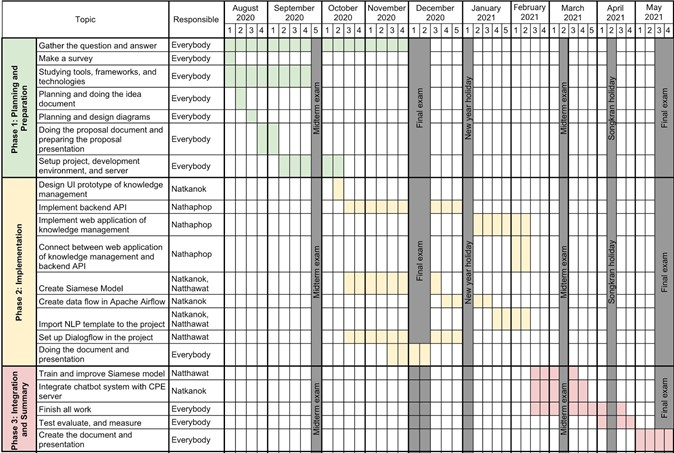
\includegraphics[width=15cm]{img/ch1/ProjectSchedule.jpg}
\captionof{table}{Task Schedule Table}
\label{fig:ProjectSchedule.jpg}
\end{figure}

%%%%%%%%%%%%%%%%%%%%%%%%%%%%%%%%%%%%%%%%%%%%%%%%%%%%%%%%%%%%
%%%%%%%%%%%%%%  Literature Review %%%%%%%%%%%%%%%%%%%%%%%%%%
%%%%%%%%%%%%%%%%%%%%%%%%%%%%%%%%%%%%%%%%%%%%%%%%%%%%%%%%%%%%
\chapter{Background Theory and Related Work}

\section{Introduction}
This chapter, we are going to demonstrate the theory, core concept, tools, and related research to be background 
and terminology before deep down into methodology and result.

\section{Theory and Core Concepts}
\subsection{Knowledge Management}
Knowledge Management is the process of creating, sharing, gathering, using and managing the knowledge 
and information in organization \cite{what_is_km}. It refers to a multidisciplinary approach to achieve organizational 
objectives by making the best use of knowledge.\\
In terms of our project, knowledge management is the website to keep the knowledge and information about 
computer engineering in question and answer format. Questions in knowledge management can group in category 
such as basic information, curriculum, frequently asked questions (FAQ), and registration. Also, in each category 
has subcategory to be more specific the question. Only staff in Computer Engineering department can use the knowledge 
management.
 
\subsection{Natural Language Processing}
Natural language processing (NLP) is a subfield of linguistics, computer science, and artificial
intelligence concerned with computers and human language interactions. The mainly how to program
computers to process and analyze large amounts of natural language data.\\
The reason for the development of NLP was that computers were originally designed to be more suited
to understand numeric information or code \cite{nlp_technology}. Which does not match the way of human
communication which relies on language and language is significantly more complex than computer-based
code. So, NLP emerged to bridge the gap in human-computer communication.\\
NLP supports both reading and listening by using other technologies such as visual recognition for
reading text and using voice recognition for listening.\\
NLP currently has a 6-step language learning process:
\begin{enumerate}
  \item Morphological Level — Understand letters. NLP will remove words in messages, find consonants,
  vowels, and spelling for the next step.
  \item Lexical Level — Understand the word after mixing the letters. It will find the meaning
  of that word to prepare for understanding the whole sentence.
  \item Syntactic Level — Understand sentences. Based on understanding the common word and structural
  order specified by experts or schemes learned.
  \item Semantic Level — Understand the context of words in a sentence. Understand the meaning of terms
  used in sentences that are outside the standard language structure.
  \item Discourse Level — Understand the syntax. Understand the effect of the previous sentence on the
  meaning of the sentence that being read. This includes understanding the order of words used in sentences
  that give different meanings.
  \item Pragmatic Level — Understand the meaning of words and sentences based on the actual situation
  or knowledge base, which may not be specified in the content. So, it can be interpreted as close to
  human beings that can always relate the new information with the old knowledge. In addition to
  understanding each point. NLP has three other language learning channels modeled after human language learning:
  \begin{itemize}
    \item Symbolic  — Symbolic is the basis of human language understanding where AI has to understand vocabulary up
    to that language's structure. Developers can now apply expert knowledge directly into AI.
    \item Statistical — After learning the basics of the language, the next step will be collect information
    on using the language in different places. The patterns were analyzed by statistical methods such as the
    frequency of words used. Find out how to sort common sentences. Then bring to synthesize new knowledge.
    This will help AI improve the language based on its current popularity. And understand the use of language
    in a particular field such as science, finance, various academic documents, etc.
    \item Connectionist AI — Connectionist AI combines a statistical language learning process with a symbolic level for complete
    communication and understanding. This is based on the Symbolic stage's actual knowledge and adapted with new
    information received from the statistical stage.
    
  \end{itemize}
\end{enumerate}

\subsection{Chatbot}
Chatbot is an artificial intelligence software used to communicate by talking with humans \cite{what_is_chatbot}.
The benefit of chatbot is chatbot can automatically communicate through messaging applications, websites, mobile apps
or through the telephone. Creating or using chatbot is fun, can be used for counselling or contact interface.\\
Chatbot might have cons as
\begin{itemize}
  \item The chatbot itself does not really understand the conversation.
  \item Scripting the chatbot with rules is fragile and hard to be fully written.
  \item Conversation quality is limited to the data.
\end{itemize}
There are two type of chatbot are IR based Chatbot and Neural Network Based Chatbot \cite{what_is_chatbot,five_types_of_chatbot}.

\subsubsection{IR Based Chatbot}
IR based chatbot uses collections of conversations in order to produce responses to conversation \cite{five_types_of_chatbot,rule_based_vs_nlp}.
Collections of conversations are stored in sequence of turns. When the chatbot receives a text,
the chatbot can produce its turn of conversation by
\begin{itemize}
  \item Using the received text to search for a turn with the closest match in the collection,
  then return the next turn as response (most initiative).
  \item Using the received text to search for a turn with the closest match in the collection,
  then return that matching turn as response (not initiative, but actually provide better result).
\end{itemize}
The turn searching is not limited to the receiving text, but rather the whole conversation so far
can be used for response searching. Downside of this approach is that the text that chatbot produces
might not be consistent. Chatbot might say something that conflicts with what the chatbot has said
before.

\subsubsection{Neural Network Based Chatbot}
Neural network based chatbot sees its response as a transformation of the incoming text. This chatbot
provides responses by training an encoder-decoder neural network with pairs of turns \cite{five_types_of_chatbot,rule_based_vs_nlp}.\\
An encoder-decoder neural network has an encoder and a decoder. The encoder transforms incoming
text into some abstract representation, and the decoder transforms that abstract representation
into response text. The encoder and the decoder usually have RNN structure, as they are capable
of handling variable length of input text and return variable length response text.

\subsection{Artificial Intelligence (AI)}
AI is a computing system that provides deep analysis like human intelligence and can produce
actionable results. For example, translation is due to the processing of incoming messages
and convert it into another language and so on.\\
AI learning is not different from human learning which “remember” and “think” like a human.
For example, children who see their parents' faces repeatedly every day and try to know whose
person is “dad” or “mother” for a long time. So children will be able to look at their face and
call “Dad” or “Mom” correctly.\\
The stimulus used to train AI is “data”, which teaches children to call “parents” must be trained
many times and must use information that has the same repetitive characteristics\cite{machine_learning_vs_deep_learning}.\\
The AI mechanism is a computer processing system, and Machine learning is a component in AI.
This machine learning has a variety of algorithms depending on the problem. Most data that used to
trend such as deep learning is an algorithm that is suitable for large complex data or Random Forests
is an algorithm that used for supervised problems, etc.\\
So, Artificial Intelligence (AI) is like a tool, a robot, or whatever the action takes place.
Let us learn from what we are interested in. The brain of AI is machine learning (ML),
learning from what we stimulate and the output is a number or code that is forwarded to display
the result or allow the AI to show action. ML can be used in various ways, from credit scoring
to analyzing a person's financial credibility, weather forecast sound analysis, or even the
translation of the language that ML is learned. It requires a programmatic mechanism or a variety
of algorithms, with data scientist designing is one of the most popular algorithms.\\
Deep learning is intended to be easy to use. However, in real work, data scientist needs to
design variables in the deep learning and need to find other algorithms as a comparison pair
to look for the most suitable algorithm in actual use.

\subsection{Deep Neural network}
Deep learning algorithms must use Artificial Neural Networks (ANN), which is the same as how
the nervous system works in the human brain \cite{machine_learning_vs_deep_learning}. These networks have neurons that
connect from the nervous system and communicate. It uses parallel processing to understand and
learn from the vast amount of information it continually receives.\\
The general principle of deep learning is to have multiple processors. The input data for each
layer is obtained through interaction with the other layers. Deep learning seeks to find deeper
relationships as the number of layers and processors in it increases. The higher the data, the
deeper and more complex (abstract).\\
The deep learning structure architecture is based on the greedy method to find things in each
layer that make deep learning more efficient than other methods. For example, early information
might learn that an incoming image consists of lines. The high floor brings together the lines
to form a rectangle. And the next layer is to find the correlation of the squares until the
computer recognizes that the image is the image of flag, etc.

\subsection{Recurrent Neural network (RNN)}
RNN is a class of artificial neural networks, but the difference is there is a connection between
each state to form a memory called “Internal memory” \cite{understand_rnn}. Unlike the feedforward
neural network, RNN can use the internal memory to process the input that is sequential data.

\begin{figure}[!h] \centering
  \setlength{\fboxrule}{0.2mm} % line border
  \setlength{\fboxsep}{0.5cm} % space between picture and line border
  \fbox{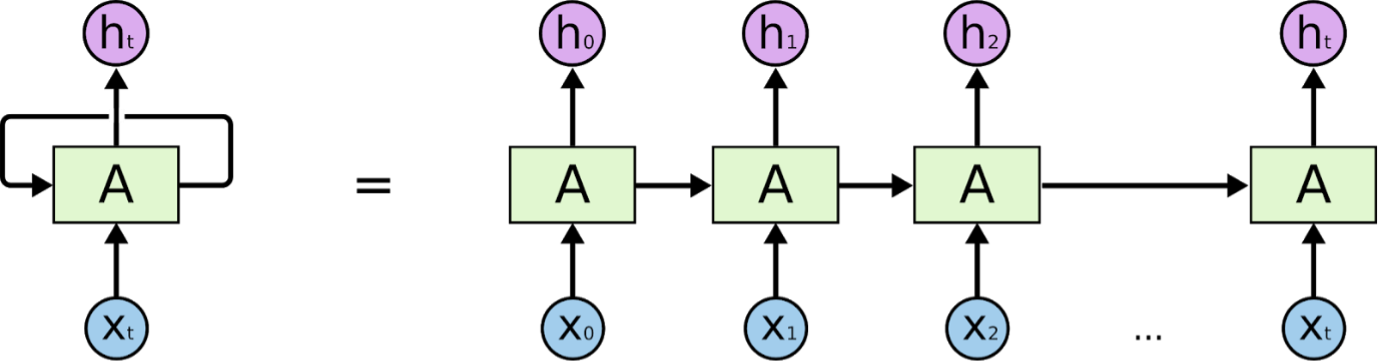
\includegraphics[width=14cm]{./img/ch2/example_rnn.png}}  %width=14cm equal to width of paragraph
  \caption{An example of RNN} % Caption under figure
  \label{fig:example_rnn} % Used for ref in paragraph
\end{figure}

Figure \ref*{fig:example_rnn} the method that RNN uses to create the internal memory is
creating a loop within it. Figure A is activated, gets the input $X_t$ in the state of time,
and output value to the hidden layer. The loop allows the information to be passed into the
next state. Therefore, the first input will affect the output in the last state.

\begin{figure}[!h] \centering
  \setlength{\fboxrule}{0.2mm} % line border
  \setlength{\fboxsep}{0.5cm} % space between picture and line border
  \fbox{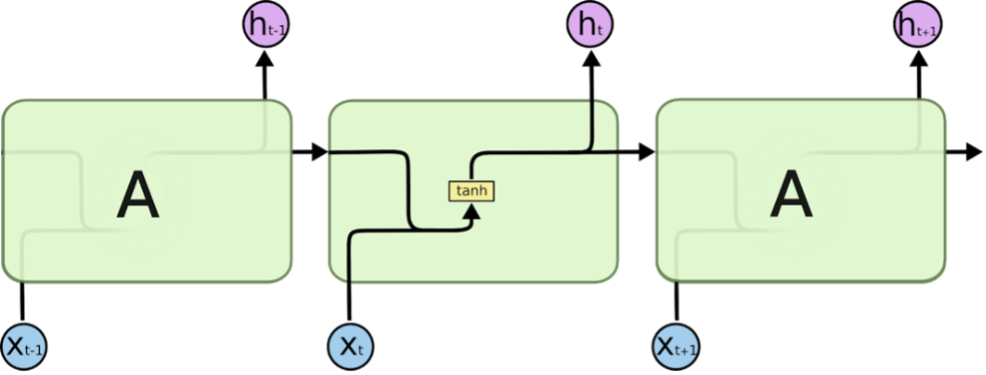
\includegraphics[width=14cm]{./img/ch2/standard_rnn.png}}  %width=14cm equal to width of paragraph
  \caption{A standard RNN method} % Caption under figure
  \label{fig:standard_rnn} % Used for ref in paragraph
\end{figure}

Inside the RNN layer, the methods are different for each type as you can see from Figure
\ref*{fig:standard_rnn}, standard RNN method. It takes the output value from the previous
state and then combines with the present state’s input. After combining the result will go
to the nonlinear function, in this case is Tanh. Then the output from this state will be
used in the later state. The figure above can transform into the formula below.

\[h_t = \Phi(Wx_t + Uh_{t-1})\]
\begin{align*}
&h(t) = \text{A hidden layer or output value of this state.}\\
&\Phi = \text{An activation function, either sigmoid function or tanh.}\\
&W = \text{The weight of the input.}\\
&x(t) = \text{A present state input.}\\
&U = \text{A hidden state matrix.}\\
&h(t-1) = \text{A hidden layer or output value of the last state.}
\end{align*}

Because of this method, many consider RNN to use whenever they need context from the past,
such as speech recognition, video analysis, and music composition.

\subsection{Long Short-Term Memory (LSTM)}
Like RNN the Long Short-Term Memory network is also a recurrent neural network but with
different architecture designs \cite{understand_rnn}, as seen in Figure \ref*{fig:lstm_arch_design}.
LSTM is specifically used to avoid the long-term dependency problem or the vanishing gradient.

\begin{figure}[!h] \centering
  \setlength{\fboxrule}{0.2mm}
  \setlength{\fboxsep}{0.5cm}
  \fbox{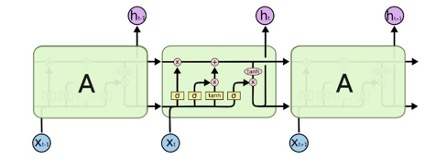
\includegraphics[width=14cm]{./img/ch2/lstm_arch_design.jpg}}
  \caption{LSTM architecture design}
  \label{fig:lstm_arch_design}
\end{figure}

The core idea of LSTM is the cell state, the horizontal line that goes between each state. The
cell state is like a bridge to carry out information from the first state throughout the model.
Besides the ability to carry information, LSTM can also manipulate the cell state by adding gates
that interact with the cell state. Each gate can alter the information on cell state like
forgetting some data or to determine which information needs to be remembered. 

\subsection{MaLSTM similarity function}
\[\exp(-\|h^{(left)} - h^{(right)}\|1)\]
In MaLSTM the identical sub-network is the way from the embedding up to the last LSTM hidden
state \cite{manhattan_lstm, what_is_embedding_matrix}. Using a LSTM to read in word-vectors that represent each
input sentence and employs final hidden state as a vector representation for each sentence.
The similarities among these representations are employed as predictors of semantic similarity.

\subsection{The architecture of Siamese Neural Network}
\begin{figure}[!h]
  \centering
  \setlength{\fboxrule}{0.2mm}
  \setlength{\fboxsep}{0.5cm}
  \fbox{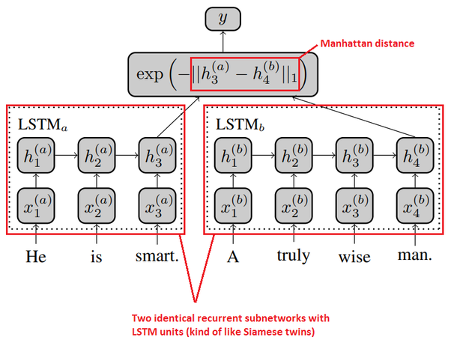
\includegraphics[width=14cm]{./img/ch2/siamese_arch.png}}
  \caption{Sample Siamese Neural Networks architecture}
  \label{fig:siamese_arch}
\end{figure}
Siamese Neural Networks is a type of neural network that contains multiple instances of the
same model and shares the same architecture and weights (twin networks) \cite{what_is_embedding_matrix, how_to_predict_questions_pair_using_malstm, introduction_siamese_network}
. This architecture shows its strength when it must learn with limited data, and we do not have a complete dataset,
for example Zero or One-shot learning tasks. They work in parallel and are responsible for creating vector
representations for the input and producing better vector representations by measuring similarities between vectors. 

\section{Tools}
Figure \ref*{fig:ch3_tools} is an overview of tools that are used in KMUTT CPE Chatbot in each subsystem.
\begin{figure}[h!]
  \centering
  \setlength{\fboxrule}{0.2mm}
  \setlength{\fboxsep}{0.5cm}
  \fbox{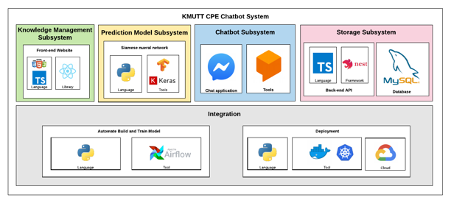
\includegraphics[width=14cm]{./img/ch2/tools.png}}
  \caption{All tools that are used in KMUTT CPE Chatbot System.}
  \label{fig:ch3_tools}
\end{figure}

\subsection{Knowledge Management Subsystem}
\subsubsection{React JS}
React is a JavaScript library, or it can be called a JavaScript Framework that we use for building
our web pages to look interesting. The strength of React that makes it worth using is that It has
a built-in caching system that makes our web pages responsive. It is very suitable for SPA
implementation. Writing React, we can also separate the elements of our web page into parts,
called as a component, and assemble it into a web page. This allows us to reuse our components
elsewhere \cite{what_is_react}. Do not waste time rewriting.

\subsubsection{GraphQL}
GraphQL is a language for accessing data (Query Language) for the use of APIs of the system \cite{what_is_graphql}
and will execute commands on the server side, also known as server-side runtime, using our defined
data structures.

\subsection{Prediction Model Subsystem}
\subsubsection{Keras}
Keras is an open-source neural network library written in python. It uses Tensorflow as one of the
backends using both CPU and GPU \cite{keras}. It is designed for a fast experiment with Deep Neural
Network. It was developed as part of the research effort of project ONEIROS (Open-ended Neuro-Electronic
Intelligent Robot Operating System). Keras library is commonly used to build neural networks such as network
layers, activation functions, optimizers, etc.

\subsubsection{TensorFlow}
Tensorflow is an open-source library for numerical computation and large-scale machine learning.
It uses Python to provide a convenient front-end API for building applications with the framework
while executing those applications in C++ \cite{what_is_tf}. TensorFlow can train and run deep neural
networks for handwritten digit classification, image recognition, word embeddings, recurrent neural
networks, and is the backend for other libraries.

\subsubsection{PyThaiNLP}
PyThaiNLP is a library package of Python languages used to process text. And language analysis,
similar to NLTK, but especially for the Thai language \cite{pythainlp}.
There are a variety of functions such as character set, Thai alphabet, Thai words,
stop words in Thai, cut Thai words, Type of grammatical words, spell check, correct words,
and much more.

\subsubsection{Apache Airflow}
Apache Airflow is an Open Source that manages various tasks by writing a Configuration in
the Python Code, which is suitable for Python programmers. Each task can see the workflow
in detail. When there is a problem, such as a bottleneck, it can be analyzed easily \cite{apache_airflow}.
We can set the working time like a Cronjob. For example, when running Job, A at 1:00 am
every day, Run Job B at 8:00 am, once a week on Sunday. Job is called DAGs
(Directed Acyclic Graphs) in Airflow is a web UI for us to monitor Task Failure
that occurred, or Duration Time caused by each work.

\subsection{Chatbot System}
\subsubsection{Dialogflow}
Dialogflow is a chatbot builder from Google which provide flexible integration to many platforms,
unique to Natural Language Processing, or NLP \cite{dialogflow}. Which means that chatbot can
accurately understand the meaning of user-typed sentences, enabling chatbot to interact with people.
Use it precisely and to the point.

\subsubsection{Facebook Messenger}
Facebook Messenger is an application through a smartphone and desktop PC. It connects information
and information, extending from the inbox system, sending messages on Facebook, and creating data
storage to facilitate communication \cite{wiki_fb_messenger}.\\
We decide this application to be our chat platform because from our survey (Figure \ref*{fig:ch3_result_survey})
through insiders and outsiders, they prefer to use the Facebook Messenger platform the most.

\begin{figure}[h!]
  \centering
  \setlength{\fboxrule}{0.2mm}
  \setlength{\fboxsep}{0.5cm}
  \fbox{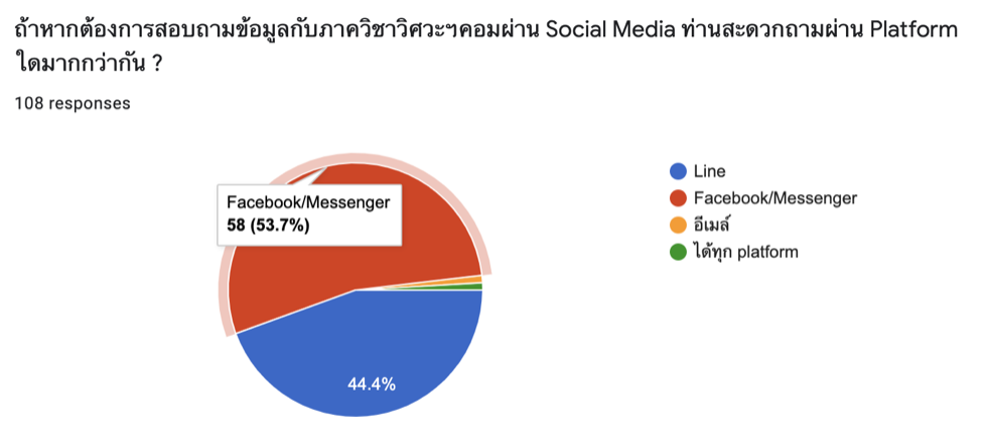
\includegraphics[width=14cm]{./img/ch2/result_survey.png}}
  \caption{The result of our survey from 108 people.}
  \label{fig:ch3_result_survey}
\end{figure}

\subsection{ Storage Subsystem}
\subsubsection{NestJS}
NestJS is a framework for building Node.js server-side applications that scalable and very
efficient \cite{nestjs_beautiful}. NestJS uses progressive JavaScript which means NestJS updated
features inside follow latest JavaScript. In addition, NestJS is very flexible from giving
freedom to easily plug the third party or another module to NestJS application. This reason
makes NestJS extensible and can be scalable to big size project.\\
Moreover, NestJS supports TypeScript and comes up with idea combination of Object-Oriented
Programming (OOP), Functional Programming (FP), and Functional Reactive Programming (FRP)
to makes more friendly to develop the application \cite{nestjs_beautiful}. Also, NestJS
provides a level of abstraction above common Node.js framework like Express or
Fastify by adding more level such as controller, provider, module, etc.

\subsubsection{MySQL}
It is a popular program used to manage database systems nowadays because of its free instruction
set. MySQL is a relational database (RDBMS: Relational Database Management System) that can
simultaneously work with multiple tables \cite{what_is_mysql}. Those tables with shared fields
MySQL are a capable database server. Standard database language like ANSI SQL
(Structured Queries Language).

\subsubsection{TypeORM}
TypeORM is Object Relational Mapping (ORM), which facilitates and simplifies database connection \cite{typeorm}.
We chose TypeORM because it supports TypeScript, which is suitable for NestJS.

\subsubsection{Bull}
Bull is a Node library that manages a queue system based on Redis, which benefits from the queue
\cite{job_queue_management_bull}. It can solve many problems elegantly, from smoothing out processing peaks to creating
robust communication channels between microservices or offloading heavy work from one server to
many smaller workers, etc.

\subsection{Deployment System}
\subsubsection{Docker}
Docker is an engine that works in a simulated environment on the server to run the required service.
It works similarly to Virtual Machines such as VMWare, VirtualBox, XEN, KVM, but the main difference
is Virtual \cite{what_is_docker}. Previously known machine It simulates the entire OS for use.

\subsubsection{Kubernetes}
Kubernetes, or k8s is an open-source platform that allows operations to Linux Containers
can be done automatically. Minimize the process of installing or extending applications
running on containers that developers have to do manually \cite{explain_kubernetes}. Or
it can be said that This enables developers to cluster a cluster of hosts
running Linux containers, and Kubernetes can quickly and efficiently manage them
for public, private, and hybrid cloud deployments.

\subsection{Languages}
\subsubsection{TypeScript}
TypeScript is a programming language that combines the capabilities that ES2015 itself has.
What is added is support for Type System and additional features such as Enum and the expanded
capabilities of object-oriented programming. TypeScript is a Babel-like transpiler \cite{what_is_ts}.
This means that the TypeScript translator will translate the code we write into JavaScript one more
time, ensuring that the result will be usable in a regular web browser.

\subsubsection{HTML}
HTML is the primary language used for writing web pages using Tag to define their display.
HTML stands for Hypertext Markup Language, where Hypertext refers to hyperlinked text.
Markup language refers to the language in which a tag is used.
HTML is defined as a language in which a tag is used to designate a web page connected
in hyperspace via Hyperlink \cite{html_basic}. It is now developed and standardized by
the World Wide Web Consortium (W3C).

\subsubsection{CSS}
CSS is a language used to decorate HTML / XHTML documents with appearance, colors, spacing,
backgrounds, borders, and more \cite{ultimate_guide_css}
. As requested, CSS stands for Cascading Style Sheets. It is a syntax-specific programming
language standardized by W3C as one of the web site decoration languages. It has been widely
popular.

\subsubsection{Python}
The Python programming language is a high-level computer programming language \cite{keras}. 
It is designed as an easy-to-read scripting language. By eliminating the complexity
of the structure and grammar of the language. In the part of converting the instruction
set to the machine, language Python has a function Interpreter is a line-by-line translation.
To enter into the processor for the computer to work as we want. Python programming language
can also be used for many types of programming. Without being limited to a particular
job (General-purpose language), it is widely used in many large global organizations such as
Google, YouTube, Instagram, Dropbox, and NASA, etc.

\section{Related Chatbot}
\subsection{Eliza}
Eliza is a rule-based chatbot. It simulates a Rogerian psychologist by reflecting the patient’s
statement back at them to continue the conversation. In the ELIZA system, there are rules. Each
rule captures some keywords. When the rules are matched, the incoming sentence is transformed
by transformation written for the rule \cite{what_is_eliza}. Each rule might have multiple
transformations to reduce repetitiveness of returning sentences.\\
Keywords in the rules are ranked. Specific meaning keywords have higher priority than general
keywords. But universal keywords such as “everybody” are exceptions. As the universal keywords
are highly probably referring to some specific event or person, universal keywords are ranked
highest.\\
Aside from rules, ELIZA also contains memory. Some rules cause ELIZA to store the topic in the
memory stack. Afterward, if no keyword match to the incoming sentence is found, content in the
memory stack is retrieved to continue the conversation.\\
Aside from rule-based transformation, there are also transformations that switch 1st person
words with 2nd persons words and vice versa.

\subsection{Parry}
Parry is a rule-based chatbot to simulate a paranoid person who is under delusion of threat
from the mafia due to Parry’s involvement in horse racing bet. Parry included a model of mental
state with 3 variables. The variables are anger, fear, and mistrust. Rules are written to
manipulate these variables \cite{parry_met_eliza}
. When Parry anger, hostile responses are made. Parry also includes a chain of topics that are
linked to mafia via horse racing. Whenever such topics are brought up for the first time,
regardless of speaker’s intention, Parry’s would feel threatened and related mental model
variables are adjusted accordingly.

\subsection{Botnoi Consulting}
Botnoi Consulting has started from Botnoi chatbot in 2016 in Line Bot Awards competition in Japan \cite{botnoi_enterprise_chatbot}.
On that time Botnoi is a chatbot on Line platform that has good relationship which can talk like
a friend and have many features such as translate, find the nearest restaurant, etc.\\
But now, Botnoi group have been upgraded to the Botnoi Consulting company. Botnoi Consulting
has developed own NLP engine in Thai language and related technology to makes many businesses
can integrate Botnoi to the system such as Botnoi API, external API integration, AI training
\& monitoring, chat analytic repots, live chat, etc. Currently, Botnoi can automatically get
input from user, provide information, make a payment, and update stock in the system without human.

\section{Related research}
\subsection{Automated Self-Learning Chatbot Initially Built as a FAQs Database Information Retrieval
System: Multi-level and Intelligent Universal Virtual Front-Office Implementing Neural Network}
This paper is about implement the multi-level virtual front office as you can see from the Figure
\ref*{fig:ch3_lr_self_learning_chatbot}. 
\begin{figure}[h!]
  \centering
  \setlength{\fboxrule}{0.2mm}
  \setlength{\fboxsep}{0.5cm}
  \fbox{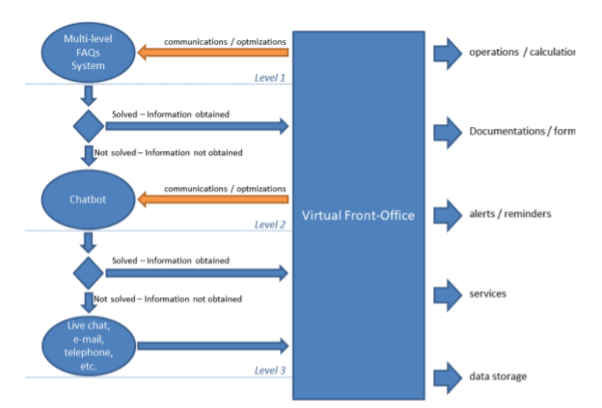
\includegraphics[width=14cm]{./img/ch2/literature_review_self_learning_chatbot.png}}
  \caption{Functional schema of Automated Self-Learning Chatbot Initially Built as a FAQs
  Database Information Retrieval System: Multi-level and Intelligent Universal Virtual
  Front-Office Implement Neural Networks.}
  \label{fig:ch3_lr_self_learning_chatbot}
\end{figure}

What we focus on from this research is about chatbot have automated self-learning from FAQs
database which is likely to our project. From Figure \ref*{fig:ch3_lr_activity_dg_self_learning_chatbot},
when there is a new question, if chatbot can answer, chatbot will send the answer to user.
But if chatbot cannot answer, the operator will answer instead and store the question FAQs
database and update A.I. engine of chatbot.\\
But the different between this research paper and our project is the chatbot and A.I. engine.
The author of research uses neural network to preprocess text before generating to AIML
pattern and create chatbot from AIML A.I. engine. While our project creates Siamese Neural
Network to pair the similarity of text between the question from user and question in
knowledge management. If both questions are the similar, our system will query the answer
from database and send answer back to the user.

\begin{figure}[h!]
  \centering
  \setlength{\fboxrule}{0.2mm}
  \setlength{\fboxsep}{0.5cm}
  \fbox{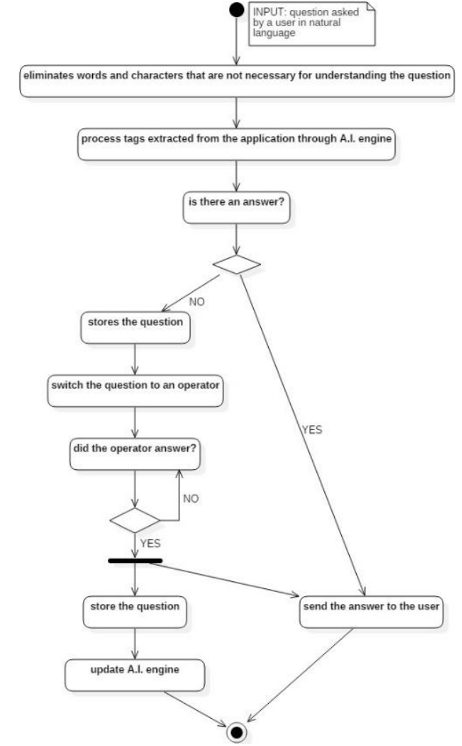
\includegraphics[width=10cm]{./img/ch2/literature_review_activity_diagram_chatbot.png}}
  \caption{Activity Diagram of Self-Learning Algorithm of Automated Self-Learning Chatbot
  Initially Built as a FAQs Database Information Retrieval System: Multi-level and Intelligent
  Universal Virtual Front-Office Implement Neural Networks.}
  \label{fig:ch3_lr_activity_dg_self_learning_chatbot}
\end{figure}

\section{Summary}
KMUTT CPE Chatbot System is a neural network based chatbot with model prediction which use
Siamese neural network to learn the similarity of question in Thai language with knowledge
management that can learn by it-self overtime not a rule based chatbot like in the existing
chatbot in the market. So, if we compare Rule-based chatbot and neural network based chatbot.
\begin{itemize}
  \item Rule-based Chatbot: The data must be entered verbatim — one sentence at a time. If the
  user asks more than that, the answer will not be answered immediately or cannot answer.
  \item Neural network based Chatbot: Understand a variety of sentence patterns. Can understand
  a wider range of questions. The users do not have to ask directly but the model can understand.
\end{itemize}
Our project can help in answering the FAQ and general inquiries of the Computer Engineering
department in KMUTT to outsiders and insiders via Facebook Messenger platform by prediction
model from knowledge management. It can reduce the over workload of KMUTT CPE staff that they
have to reply to the same answer to same questions to insiders or outsiders as quickly as they
can and repeatedly every day. So, if we compare or solution with the existing solution which is
the CPE staff have to answer by themselves (Table \ref*{table:ch3_solution_compare}).
\begin{figure}[h!]
  \centering
  \fbox{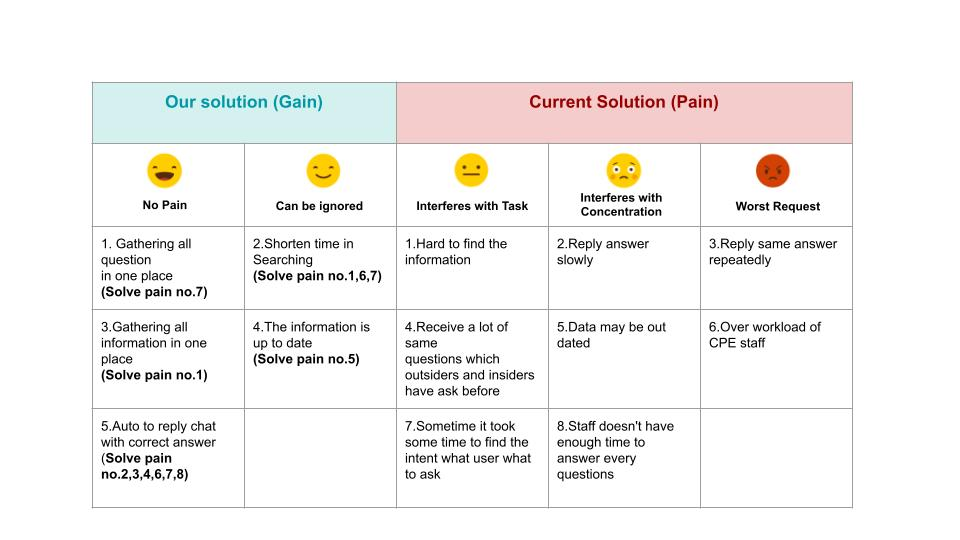
\includegraphics[width=15cm]{./img/ch2/solution_compare.jpg}}
  \captionof{table}{Compare KMUTT CPE chatbot with the existing solution which is the CPE
  staff have to answer by themselves.}
  \label{table:ch3_solution_compare}
\end{figure}

Overall KMUTT CPE Chatbot system can reduce the workload of document workers and reduce human
error when answering the question. Also, can reply to outsiders and insiders correctly and
immediately. It will serve either the computer engineering insiders or people interested in
computer engineering to answer the question about the department and CPE staff can use
knowledge management to manage FAQ in the department.
Moreover, our chatbot systems can scalable, the chatbot can automatically build models
when knowledge management receives new data.

%%%%%%%%%%%%%%%%%%%%%%%%%%%%%%%%%%%%%%%%%%%%%%%%%%%%%
%%%%%%%%%%%%%%%%%%%%%%%%%%%%%%%%%%%%%%%%%%%%%%%%%%%%%
\chapter{Proposed Work}

\section{Introduction}
This chapter demonstrates our plan and idea to be method or approach to reach the goal. In this chapter consists of system architecture, workload of each person, planning diagram such as use case, sequence diagram, etc., data management, design of key processing algorithms, and evaluation plans to evaluate our project.

\section{System Architecture}
After planning and discussion with advisor, KMUTT CPE Chatbot System can be divide into 4 subsystems which consists of knowledge management subsystem, prediction model subsystem, chatbot subsystem, and storage subsystem
\begin{figure}[h!]
	\centering
	\setlength{\fboxrule}{0.2mm}
	\setlength{\fboxsep}{0.5cm}
	\fbox{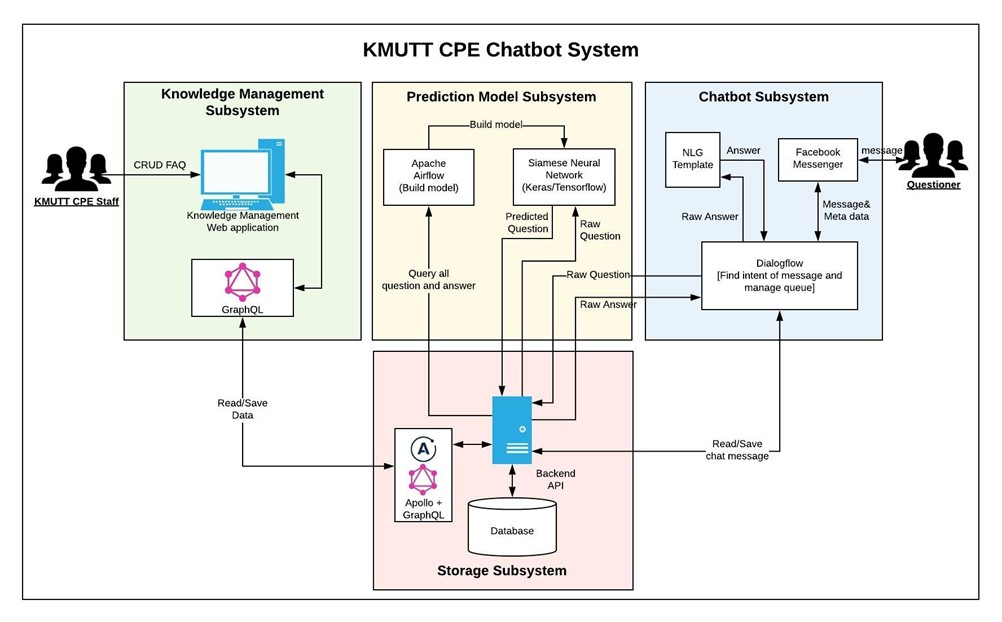
\includegraphics[width=10cm]{img/ch3/System Architecture.jpg}}
	\caption{System architecture of KMUTT CPE Chatbot System}
	\label{fig:System architecture of KMUTT CPE Chatbot System}
\end{figure}

\begin{description}
	\item [Knowledge Management Subsystem]
	\hfill \\The knowledge management subsystem is related to knowledge management for the Computer Engineering department, allowing the staff to manage the FAQ. Also, FAQ from knowledge management will be the data for building the model.\\
	This subsystem contains only web applications based on a web browser for KMUTT CPE staff. Our group will build the knowledge management web application by using the TypeScript language and React library. The web application also read and save to the database through the GraphQL gateway to backend API.
	\item [Prediction Model Subsystem]
	\hfill \\The prediction model subsystem is related to the chatbot's prediction model and includes the automated build model.\\
	This subsystem consists of Apache Airflow and Siamese Neural Network. Apache Airflow is used to automate build the Siamese model. It will query all questions and answers from the backend API and build the model in a schedule. While Siamese Neural Network input as a sequence of questions from the questioner, then pair with the FAQ in knowledge management and then return the related question.
	\item [Chatbot Subsystem]
	\hfill \\Chatbot subsystem is related to the managing queue of chat from many users, chat flow and intent message.\\
	This subsystem consists of Facebook Messenger, Dialogflow, and NLG Template. Facebook Messenger is a chat platform where people can ask their question, and this platform will be connected to Dialogflow. Dialogflow will manage the chat flow and chat queue from Facebook Messenger and intent to message that the message is a question or common message like greeting. If the message is common message, Dialogflow will automatically replied with a common answer. But if it is a question, Dialogflow will send the question to the backend API to get the answer back.
	\item [Storage Subsystem]
	\hfill \\The storage subsystem is related to managing data and providing API for each subsystem.\\
	Storage subsystem consists of a database and backend API. Our database is MySQL, and it keeps all data from each subsystem, either knowledge management subsystem or chatbot subsystem. But both subsystems need to save the data into the database through the backend API. The backend API provides the restful API and GraphQL for all subsystems to query, update, and delete data. Moreover, the back-end API provides an API to get a question from Dialogflow and manage the question in the queue to send a question to the prediction model and return an answer from knowledge management.
\end{description}
\section{System Requirements}
	\subsection{Knowledge Management Subsystem}
	\begin{itemize}
		\item Deploying new knowledge management for Computer Engineering department
		\item KMUTT CPE Staff can create, update, read, and delete the FAQ in Knowledge management.
		\item Knowledge management subsystem can save the data in the database through the storage subsystem.
	\end{itemize}
\emph{workload}
\begin{table}[h]
	\centering
	\caption{Workload of knowledge management subsystem}
	\label{tab:Workload of knowledge management subsystem}
\begin{adjustbox}{width=\textwidth}
\begin{tabular}{lp{0.25\linewidth}l}
		\rowcolor[HTML]{5B9BD5} 
		Task                                                                              & Responsibility \\
		\rowcolor[HTML]{DEEAF6} 
		Design user interface                                                             & Natkanok       \\
		\rowcolor[HTML]{FFFFFF} 
		Setup environment and dependency                                                  & Nathaphop      \\
		\rowcolor[HTML]{DEEAF6} 
		Create each component of website such as button, navbar, input   box, table, etc. & Nathaphop      \\
		Implement web page follow the user interface   design                             & Nathaphop      \\
		\rowcolor[HTML]{DEEAF6} 
		Connect the website to backend API with   GraphQL                                 & Nathaphop      \\
		Test function and website interface in each   browser                             & Nathaphop      
	\end{tabular}
\end{adjustbox}
\end{table}

	\subsection{Prediction Model Subsystem}
	\begin{itemize}
		\item Use the FAQ data from knowledge management to build the model
		\item The model has input as a sequence of question from the questioner, then pairs with the FAQ in knowledge management, and then returns the related question back.
		\item Automate build model and deploy
	\end{itemize}
\emph{workload}
\begin{table}[h]
	\centering
	\caption{Workload of prediction model subsystem}
	\label{tab:Workload of prediction model subsystem}
\begin{adjustbox}{width=\textwidth}
\begin{tabular}{lp{0.6\linewidth}l}
		\rowcolor[HTML]{5B9BD5} 
		Task                                        & Responsibility      \\
		\rowcolor[HTML]{DEEAF6} 
		Gathering Pantip data to create data corpus & Natkanok            \\
		Manually pair similar text                  & Natkanok            \\
		\rowcolor[HTML]{DEEAF6} 
		Preprocess and clean data                   & Natkanok            \\
		Build the model                             & Natkanok            \\
		\rowcolor[HTML]{DEEAF6} 
		Train model                                 & Natkanok, Natthawat \\
		Evaluate and tuning model                   & Natkanok, Natthawat 
	\end{tabular}
\end{adjustbox}
\end{table}

	\subsection{Chatbot Subsystem}
	\begin{itemize}
		\item Chatbot subsystem can manage queues and chat flow.
		\item Chatbot subsystem must connect with Facebook Messenger.
		\item Chatbot subsystem can get the question from people and can reply answer from knowledge management back.
		\item Chatbot subsystem can keep log messages in the database through storage subsystem.
	\end{itemize}
\emph{workload}
\begin{table}[h]
	\centering
	\caption{Workload of chatbot subsystem}
	\label{tab:Workload of chatbot subsystem}
\begin{adjustbox}{width=\textwidth}
\begin{tabular}{ll}
		\rowcolor[HTML]{5B9BD5} 
		Task                                                                                       & Responsibility \\
		\rowcolor[HTML]{DEEAF6} 
		Create app in Facebook developer and write app review                                      & Natthawat      \\
		Write privacy policy and term of service in   Facebook developer                           & Natthawat      \\
		\rowcolor[HTML]{DEEAF6} 
		Create business account                                                                    & Natthawat      \\
		Write data protection officer contact   information                                        & Natthawat      \\
		\rowcolor[HTML]{DEEAF6} 
		Generate token to Facebook and connect Facebook   webhook to Dialogflow                    & Natthawat      \\
		Create agent in Dialogflow to makes it be able   to handle both Thai and English languages & Natthawat      \\
		\rowcolor[HTML]{DEEAF6} 
		Connect webhook Dialogflow to our system                                                   & Natthawat      
	\end{tabular}
\end{adjustbox}
\end{table}

	\subsection{Storage Subsystem}
	\begin{itemize}
		\item Storage subsystem can manage a queue of questions from the chatbot subsystem to the prediction model subsystem.
		\item Storage subsystem provides API to the knowledge management subsystem and chatbot subsystem.
		\item Storage subsystem can send all questions to the prediction model subsystem for building the model.
	\end{itemize}
\emph{workload}
\begin{table}[h]
	\centering
	\caption{Workload of storage subsystem}
	\label{tab:Workload of storage subsystem}
\begin{adjustbox}{width=\textwidth}
\begin{tabular}{lp{0.5\linewidth}l}
		\rowcolor[HTML]{5B9BD5} 
		Task                                               & Responsibility                 \\
		\rowcolor[HTML]{DEEAF6} 
		Design database schema                             & Nathaphop                      \\
		Planning code structure                            & Nathaphop                      \\
		\rowcolor[HTML]{DEEAF6} 
		Setup environment and dependency                   & Nathaphop                      \\
		Implement entities object of each table            & Nathaphop                      \\
		\rowcolor[HTML]{DEEAF6} 
		Provide necessary restful API and GraphQL          & Nathaphop                      \\
		Doing unit test and integrate test                 & Nathaphop                      \\
		\rowcolor[HTML]{DEEAF6} 
		Integrate all subsystems and deploy to environment & Nathaphop, Natkanok, Natthawat 
	\end{tabular}
\end{adjustbox}
\end{table}

\pagebreak

\section{Use case diagram}
Figure ~\ref*{fig:use case diagram} shows the main things that the KMUTT CPE staff and questioner can do with the KMUTT CPE Chatbot System. Knowledge management is used by KMUTT CPE staff only.
\begin{figure}[!h]
	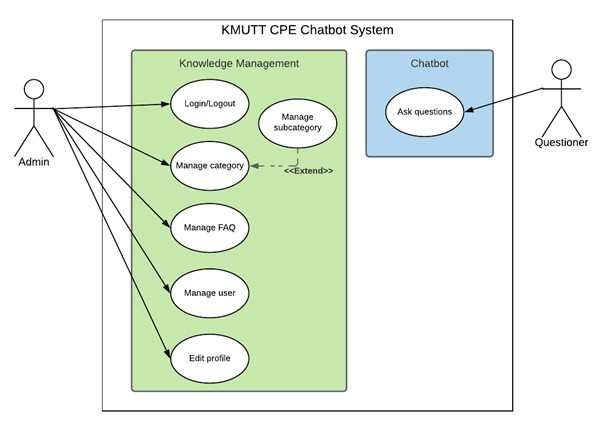
\includegraphics[width=14cm]{img/ch3/use case diagram.jpg}
	\caption{Use case of KMUTT CPE Chatbot}\label{fig:use case diagram}
\end{figure}

\section{Use case narrative}
\subsection{Login}
\underline{Actor}: Admin\\
\underline{Goal}: Admin can login to the system\\
\underline{Precondition}: Register username and password by root user\\
\underline{Main Success Scenario}:
\begin{enumerate}[label={\arabic*.}]
	\item Admin inputs valid username and password in input box        
	\item Admin clicks login button
	\item Redirect to knowledge management workspace
\end{enumerate}
\underline{Extension a}:
\begin{enumerate}[label={\arabic*.}]
	\item Admin inputs valid username and password in input box        
	\item Admin clicks login button
	\item Website displays the error message of incorrect username or password
\end{enumerate}
\underline{Postcondition}: 
\begin{enumerate}[label={\arabic*.}]
	\item Admin can access feature inside knowledge management
\end{enumerate}

\subsection{Logout}
\underline{Actor}: Admin\\
\underline{Goal}: Admin can logout from the system\\
\underline{Precondition}: Admin need to login to the system first\\
\underline{Main Success Scenario}:
\begin{enumerate}[label={\arabic*.}]
	\item Admin clicks logout button      
	\item Redirect to home page
\end{enumerate}
\underline{Postcondition}: 
\begin{enumerate}[label={\arabic*.}]
	\item Admin can access feature inside knowledge management
\end{enumerate}

\subsection{Edit Profile}
\underline{Actor}: Admin\\
\underline{Goal}: Admin can edit their profile\\
\underline{Precondition}: Admin need to login to the system first\\
\underline{Main Success Scenario}:
\begin{enumerate}[label={\arabic*.}]
	\item Admin clicks edit profile       
	\item Redirect to edit profile page
	\item Admin edits their own profile such as name or password
	\item Admin clicks save and confirm the edit action
\end{enumerate}
\underline{Postcondition}: 
\begin{enumerate}[label={\arabic*.}]
	\item Admin can access feature inside knowledge management
\end{enumerate}

\subsection{Read category}
\underline{Actor}: Admin\\
\underline{Goal}: Admin can read category data\\
\underline{Precondition}: Admin need to login to the system first\\
\underline{Main Success Scenario}:
\begin{enumerate}[label={\arabic*.}]
	\item Admin goes to category management page      
	\item Admin can read all categories
\end{enumerate}
\underline{Postcondition}: -

\subsection{Create category}
\underline{Actor}: Admin\\
\underline{Goal}: Admin can create category data\\
\underline{Precondition}: Admin need to login to the system first\\
\underline{Main Success Scenario}:
\begin{enumerate}[label={\arabic*.}]
	\item Admin goes to category management page
	\item Admin clicks create category button
	\item Admin inputs category name in input box
	\item Admin clicks create button
	\item Admin confirm create action
\end{enumerate}
\underline{Postcondition}: 
\begin{enumerate}[label={\arabic*.}]
	\item Admin can see the updated category list and can select category when manage the question
	\item Websites contains new category
\end{enumerate}

\subsection{Edit category}
\underline{Actor}: Admin\\
\underline{Goal}: Admin can edit category data\\
\underline{Precondition}: Admin need to login to the system first\\
\underline{Main Success Scenario}:
\begin{enumerate}[label={\arabic*.}]
	\item Admin goes to category management page
	\item Admin clicks edit category button
	\item Admin edits category name
	\item Admin clicks save button
	\item Admin confirm edit action
\end{enumerate}
\underline{Postcondition}: 
\begin{enumerate}[label={\arabic*.}]
	\item Admin can see the updated category list
	\item Websites update the category
\end{enumerate}

\subsection{Remove category}
\underline{Actor}: Admin\\
\underline{Goal}: Admin can remove category\\
\underline{Precondition}: Admin need to login to the system first\\
\underline{Main Success Scenario}:
\begin{enumerate}[label={\arabic*.}]
	\item Admin goes to category management page
	\item Admin clicks remove category button
	\item Admin confirm remove action
\end{enumerate}
\underline{Postcondition}: 
\begin{enumerate}[label={\arabic*.}]
	\item Admin can see the updated category list
	\item Websites remove that category, subcategories, and questions inside that category
\end{enumerate}

\subsection{Read subcategory}
\underline{Actor}: Admin\\
\underline{Goal}: Admin can read subcategory data in each category\\
\underline{Precondition}: Admin need to login to the system first\\
\underline{Main Success Scenario}:
\begin{enumerate}[label={\arabic*.}]
	\item Admin goes to category management page
	\item Admin clicks to category that interested
	\item Admin can read all subcategories inside that category
\end{enumerate}
\underline{Postcondition}: -

\subsection{Create subcategory}
\underline{Actor}: Admin\\
\underline{Goal}: Admin can create subcategory\\
\underline{Precondition}: Admin need to login to the system first\\
\underline{Main Success Scenario}:
\begin{enumerate}[label={\arabic*.}]
	\item Admin goes to category management page
	\item Admin clicks to the category that want to add a new subcategory
	\item Admin clicks create new subcategory button
	\item Admin inputs subcategory name in input box
	\item Admin clicks create button
	\item Admin confirm create action
\end{enumerate}
\underline{Postcondition}: 
\begin{enumerate}[label={\arabic*.}]
	\item Admin can see the updated subcategory list and can select subcategory when manage the question
	\item Websites contains new subcategory
\end{enumerate}

\subsection{Edit subcategory}
\underline{Actor}: Admin\\
\underline{Goal}: Admin can edit subcategory\\
\underline{Precondition}: Admin need to login to the system first\\
\underline{Main Success Scenario}:
\begin{enumerate}[label={\arabic*.}]
	\item Admin goes to category management page
	\item Admin clicks category that have subcategory that want to edit
	\item Admin clicks edit subcategory button
	\item Admin edits subcategory name
	\item Admin clicks save button
	\item Admin confirm edit action
\end{enumerate}
\underline{Postcondition}: 
\begin{enumerate}[label={\arabic*.}]
	\item Admin can see the updated subcategory list
	\item Websites update the subcategory
\end{enumerate}

\subsection{Remove subcategory}
\underline{Actor}: Admin\\
\underline{Goal}: Admin can remove subcategory\\
\underline{Precondition}: Admin need to login to the system first\\
\underline{Main Success Scenario}:
\begin{enumerate}[label={\arabic*.}]
	\item Admin goes to category management page
	\item Admin clicks category that have subcategory that want to remove
	\item Admin clicks remove subcategory button
	\item Admin confirm delete action
\end{enumerate}
\underline{Postcondition}: 
\begin{enumerate}[label={\arabic*.}]
	\item Admin can see the updated category list
	\item Websites remove all of questions in that subcategory
\end{enumerate}

\subsection{Read FAQ}
\underline{Actor}: Admin\\
\underline{Goal}: Admin can read question in knowledge management\\
\underline{Precondition}: Admin need to login to the system first\\
\underline{Main Success Scenario}:
\begin{enumerate}[label={\arabic*.}]
	\item Admin goes to question management page
	\item Admin selects the category of question that want to read
	\item Admin can see the list of questions and can click to the question that want to read
\end{enumerate}
\underline{Postcondition}: 
\begin{enumerate}[label={\arabic*.}]
	\item Admin can see information of that question, consists of question, answer, category, subcategory, last editor, and last updated.
\end{enumerate}

\subsection{Create FAQ}
\underline{Actor}: Admin\\
\underline{Goal}: Admin can create question in knowledge management\\
\underline{Precondition}: Admin need to login to the system first\\
\underline{Main Success Scenario}:
\begin{enumerate}[label={\arabic*.}]
	\item Admin goes to question management page
	\item Admin clicks to create new question
	\item Admin selects category and subcategory
	\item Admin inputs question and answer
	\item Admin clicks create button
	\item Admin confirm create action
\end{enumerate}
\underline{Postcondition}: 
\begin{enumerate}[label={\arabic*.}]
	\item Admin can see the updated question list
\end{enumerate}

\subsection{Edit FAQ}
\underline{Actor}: Admin\\
\underline{Goal}: Admin can edit question in knowledge management\\
\underline{Precondition}: Admin need to login to the system first\\
\underline{Main Success Scenario}:
\begin{enumerate}[label={\arabic*.}]
	\item Admin goes to question management page
	\item Admin selects the category of question that want to edit
	\item Admin selects the question that wants to edit
	\item Admin edits the question
	\item Admin click saves
	\item Admin confirm edit action
\end{enumerate}
\underline{Postcondition}: 
\begin{enumerate}[label={\arabic*.}]
	\item Admin can see the updated question list
\end{enumerate}

\subsection{Remove FAQ}
\underline{Actor}: Admin\\
\underline{Goal}: Admin can remove question in knowledge management\\
\underline{Precondition}: Admin need to login to the system first\\
\underline{Main Success Scenario}:
\begin{enumerate}[label={\arabic*.}]
	\item Admin goes to question management page
	\item Admin selects the category of question that want to remove
	\item Admin selects the question that wants to remove
	\item Admin confirm delete action
\end{enumerate}
\underline{Postcondition}: 
\begin{enumerate}[label={\arabic*.}]
	\item Admin can see the updated question list
	\item Websites contains new category
\end{enumerate}

\subsection{Read user}
\underline{Actor}: Admin\\
\underline{Goal}: Admin can read user information in knowledge management\\
\underline{Precondition}: Admin need to login to the system first\\
\underline{Main Success Scenario}:
\begin{enumerate}[label={\arabic*.}]
	\item Admin goes to user management page
	\item Admin can see the list of users and can click user that want to read information
\end{enumerate}
\underline{Postcondition}: 
\begin{enumerate}[label={\arabic*.}]
	\item Admin can read information of that user.
\end{enumerate}

\subsection{Create user}
\underline{Actor}: Admin\\
\underline{Goal}: Admin can create new user account\\
\underline{Precondition}: Admin need to login to the system first\\
\underline{Main Success Scenario}:
\begin{enumerate}[label={\arabic*.}]
	\item Admin goes to user management page
	\item Admin clicks create new user button
	\item Admin input username that doesn’t exist in the system
	\item Admin input password, and confirmed password
	\item Admin input name of the user
	\item Admin clicks create user and confirm create action
\end{enumerate}
\underline{Extension a}:
\begin{enumerate}[label={\arabic*.}]
	\item Admin goes to user management page
	\item Admin clicks create new user button
	\item Admin input username that already exists in the system
	\item Admin input password, and confirmed password
	\item Admin input name of the user
	\item Admin clicks create
	\item Websites display error message of user have already exists
\end{enumerate}
\underline{Postcondition}: 
\begin{enumerate}[label={\arabic*.}]
	\item Admin can see the updated list of users
	\item Should not create the username that already exists in the system
\end{enumerate}

\subsection{Edit user}
\underline{Actor}: Admin\\
\underline{Goal}: Admin can create new user account\\
\underline{Precondition}: Admin need to login to the system first\\
\underline{Main Success Scenario}:
\begin{enumerate}[label={\arabic*.}]
	\item Admin goes to user management page
	\item Admin clicks edit button on the account that want to edit
	\item Admin edits password or name
	\item Admin click saves and confirm edit action
\end{enumerate}
\underline{Postcondition}: 
\begin{enumerate}[label={\arabic*.}]
	\item Admin can see the updated list of users
\end{enumerate}

\subsection{Remove user}
\underline{Actor}: Admin\\
\underline{Goal}: Admin can remove user account\\
\underline{Precondition}: Admin need to login to the system first\\
\underline{Main Success Scenario}:
\begin{enumerate}[label={\arabic*.}]
	\item Admin goes to user management page
	\item Admin clicks remove button on the account that want to remove
	\item Admin click confirm remove action
\end{enumerate}
\underline{Extension a}:
\begin{enumerate}[label={\arabic*.}]
	\item Admin goes to user management page
	\item Admin clicks remove button on the own account
	\item Website display error message causes from delete own account
\end{enumerate}
\underline{Postcondition}: 
\begin{enumerate}[label={\arabic*.}]
	\item Admin can see the updated list of users
\end{enumerate}

\pagebreak

\section{Workflow}
\subsection{The sequence diagram workflow of chat message}
Figure ~\ref*{fig:Sequence diagram workflow of chat message} illustrates the chat workflow starting from a question from questioner until reply answer in knowledge management back. When the questioner sends the message via Facebook Messenger, the message will be sent directly to Dialogflow.\\
Dialogflow will manage the chat queue, save the meta of the questioner and message to the database, and then find the intended message to identify the message that it is a question or common message like a greeting message. If the message is common, Dialogflow will automatically be replied with a common message. But if it is a question, Dialogflow will send the message to the backend API to get the answer to reply.\\
The backend API will manage the queue of questions from Dialogflow before sending it to the Siamese model. The Siamese model will pair the question from the questioner and all questions in FAQ, then return the related question to the Backend API.\\
After the backend API gets a related question (or a predicted question), the back-end API will query the raw answer from the database and return to the Dialogflow. Dialogflow will change answers into human speech with an NLP template before replying to the questioner.
\begin{figure}[!h]
	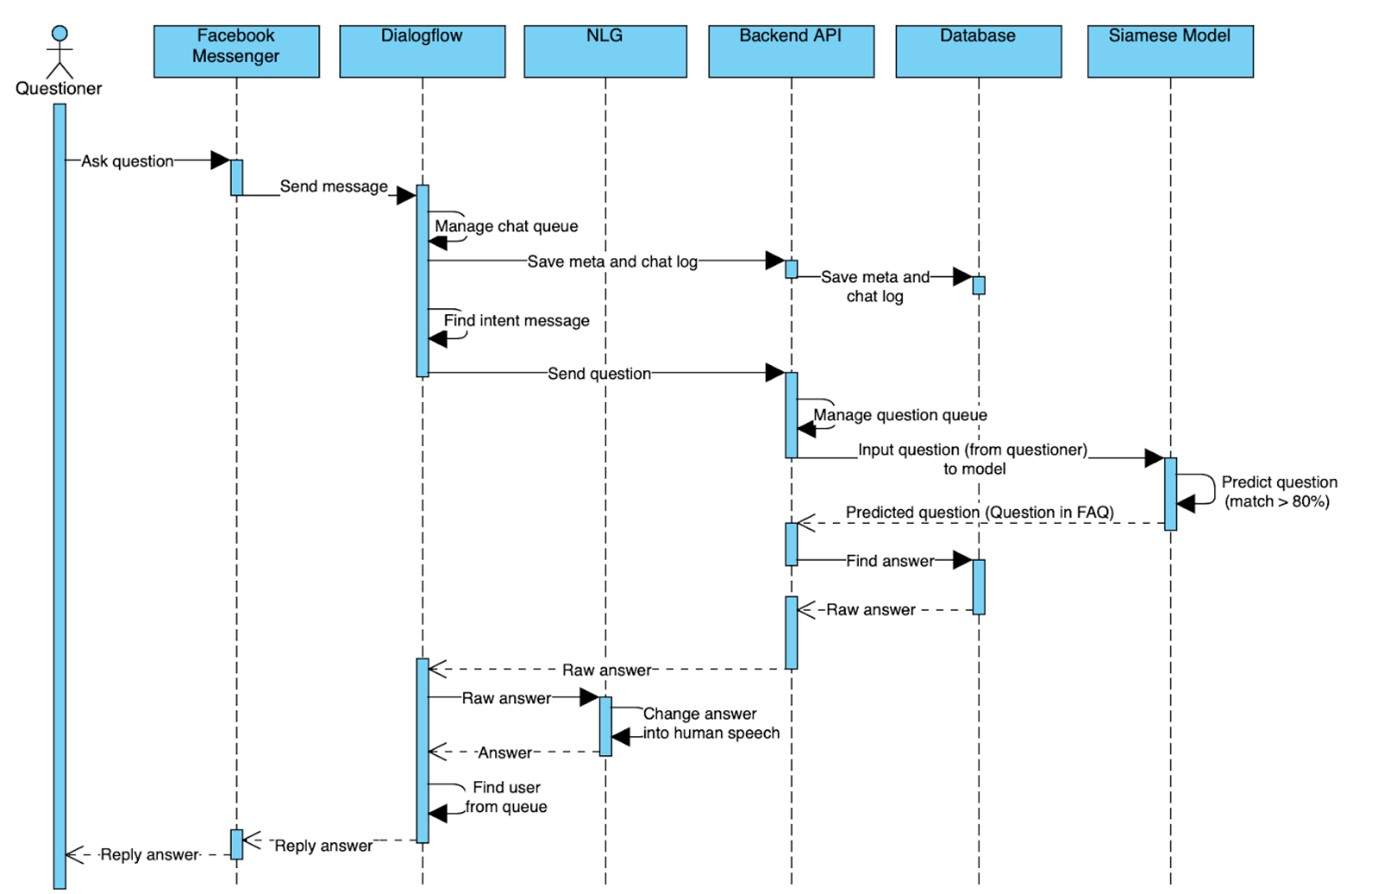
\includegraphics[width=14cm]{img/ch3/sequence diagram of chat message.jpg}
	\caption{Sequence diagram workflow of chat message}\label{fig:Sequence diagram workflow of chat message}
\end{figure}

\pagebreak

\subsection{The sequence diagram of automate build model}
Figure ~\ref*{fig:Sequence diagram of automate building and deploy model.} illustrates the workflow of automating build prediction models. Apache Airflow automatically gets the question from the back-end API, builds the model, and deploys on Google Cloud
\begin{figure}[!h]
	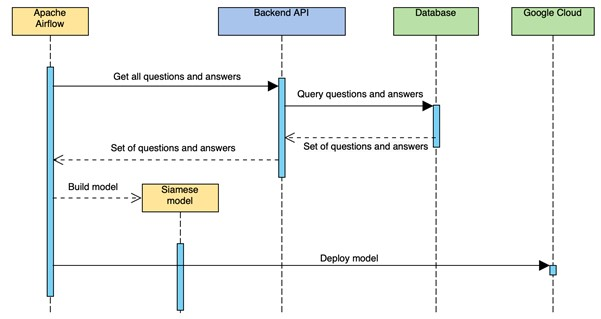
\includegraphics[width=14cm]{img/ch3/sequence diagram of automate build model.jpg}
	\caption{Sequence diagram of automate building and deploy model.}\label{fig:Sequence diagram of automate building and deploy model.}
\end{figure}

\section{Database Schema}
\begin{figure}[!h]
	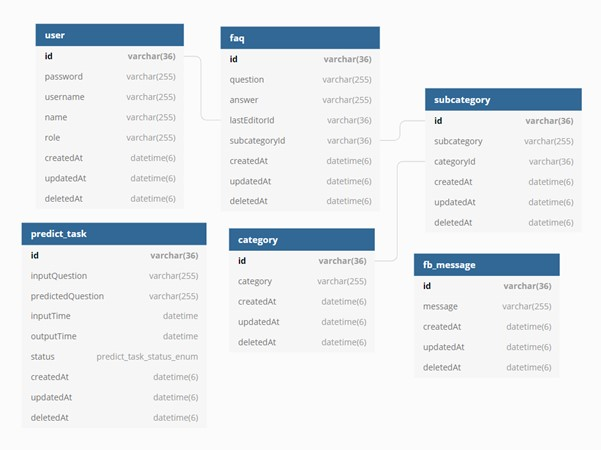
\includegraphics[width=14cm]{img/ch3/Database Schema.jpg}
	\caption{ER Diagram illustrates database schema.}\label{fig:ER Diagram illustrates database schema.}
\end{figure}

\pagebreak

\textbf{user} - User that can access knowledge management system.

\begin{table}[ht]
	\caption{User entity description table.}
	\label{tab:User entity description table}
\begin{adjustbox}{width=\textwidth}
\begin{tabular}{llp{0.6\linewidth}l}
\rowcolor[HTML]{5B9BD5} 
Attribute & Type     & Description                                                                                                   \\
\rowcolor[HTML]{DEEAF6} 
id (PK)   & Varchar  & Id of user table                                                                                              \\
username  & Varchar  & Username of account                                                                                           \\
\rowcolor[HTML]{DEEAF6} 
password  & Varchar  & Password of account                                                                                           \\
name      & Varchar  & Name of the account                                                                                           \\
\rowcolor[HTML]{DEEAF6} 
role      & Varchar  & Role of the account. Currently have only one role which is admin.                                             \\
createdAt & Datetime & Created time of the row   data                                                                                \\
\rowcolor[HTML]{DEEAF6} 
updatedAt & Datetime & Updated time of the row data                                                                                  \\
deletedAt & Datetime & Used soft delete method   to be able to recover the data. This column used to keep the deleted time of   data
\end{tabular}
\end{adjustbox}
\end{table}

\textbf{faq} - Frequently asked question that admin create through the knowledge management system.
\begin{table}[ht]
	\caption{FAQ entity description table.}
	\label{tab:FAQ entity description table.}
\begin{adjustbox}{width=\textwidth}
\begin{tabular}{llp{0.5\linewidth}l}
\rowcolor[HTML]{5B9BD5} 
Attribute          & Type     & Description                                                                                                   \\
\rowcolor[HTML]{DEEAF6} 
id (PK)            & Varchar  & Id of faq table                                                                                               \\
question           & Varchar  & Frequently asked   question                                                                                   \\
\rowcolor[HTML]{DEEAF6} 
answer             & Varchar  & Answer of the question                                                                                        \\
lastEditorId (FK)  & Varchar  & Name of the account                                                                                           \\
\rowcolor[HTML]{DEEAF6} 
subcategoryId (FK) & Varchar  & Subcategory of the question. Also, use this subcategory id to track   the category.                           \\
createdAt          & Datetime & Created time of the row   data                                                                                \\
\rowcolor[HTML]{DEEAF6} 
updatedAt          & Datetime & Updated time of the row data                                                                                  \\
deletedAt          & Datetime & Used soft delete method   to be able to recover the data. This column used to keep the deleted time of data
\end{tabular}
\end{adjustbox}
\end{table}

\textbf{category} - Category of the question.
\begin{table}[ht]
	\caption{Category entity description table.}
	\label{tab:Category entity description table.}
\begin{adjustbox}{width=\textwidth}
\begin{tabular}{llp{0.6\linewidth}l}
\rowcolor[HTML]{5B9BD5} 
Attribute & Type     & Description                                                                                                 \\
\rowcolor[HTML]{DEEAF6} 
id (PK)   & Varchar  & Id of category table                                                                                        \\
category  & Varchar  & Category of question                                                                                        \\
\rowcolor[HTML]{DEEAF6} 
createdAt & Datetime & Created time of the row data                                                                                \\
updatedAt & Datetime & Updated time of the row   data                                                                              \\
\rowcolor[HTML]{DEEAF6} 
deletedAt & Datetime & Used soft delete method to be able to recover the data. This column   used to keep the deleted time of data
\end{tabular}
\end{adjustbox}
\end{table}

\pagebreak

\textbf{subcategory} - Subcategory of the question.
\begin{table}[ht]
	\caption{Subcategory entity description table.}
	\label{tab:Subcategory entity description table.}
\begin{adjustbox}{width=\textwidth}
\begin{tabular}{llp{0.6\linewidth}l}
\rowcolor[HTML]{5B9BD5} 
Attribute       & Type     & Description                                                                                                   \\
\rowcolor[HTML]{DEEAF6} 
id (PK)         & Varchar  & Id of subcategory table                                                                                       \\
subcategory     & Varchar  & Subcategory of question                                                                                       \\
\rowcolor[HTML]{DEEAF6} 
categoryId (FK) & Varchar  & Category of subcategory                                                                                       \\
createdAt       & Datetime & Created time of the row   data                                                                                \\
\rowcolor[HTML]{DEEAF6} 
updatedAt       & Datetime & Updated time of the row data                                                                                  \\
deletedAt       & Datetime & Used soft delete method   to be able to recover the data. This column used to keep the deleted time of   data
\end{tabular}
\end{adjustbox}
\end{table}

\textbf{predict\_task} - Message that going to predict in prediction model. Used to keep log of question message and predict task.
\begin{table}[ht]
	\caption{Prediction model entity description table.}
	\label{tab:Prediction model entity description table.}
\begin{adjustbox}{width=\textwidth}
\begin{tabular}{llp{0.6\linewidth}l}
\rowcolor[HTML]{5B9BD5} 
Attribute         & Type     & Description                                                                                                 \\
\rowcolor[HTML]{DEEAF6} 
id (PK)           & Varchar  & Id of predict\_task table                                                                                   \\
inputQuestion     & Varchar  & Subcategory of question                                                                                     \\
\rowcolor[HTML]{DEEAF6} 
predictedQuestion & Varchar  & Category of subcategory                                                                                     \\
inputTime         & Datetime & Input time that the   question message go to compare in the prediction model                                \\
\rowcolor[HTML]{DEEAF6} 
outputTime        & Datetime & Output time from the prediction model                                                                       \\
status            & Enum     & Status of the task,   ‘NEW’, ‘IN\_PROCESS’, ‘SUCCESS’, ‘FAILURE’.                                           \\
\rowcolor[HTML]{DEEAF6} 
createdAt         & Datetime & Created time of the row data                                                                                \\
updatedAt         & Datetime & Updated time of the row   data                                                                              \\
\rowcolor[HTML]{DEEAF6} 
deletedAt         & Datetime & Used soft delete method to be able to recover the data. This column   used to keep the deleted time of data
\end{tabular}
\end{adjustbox}
\end{table}

\textbf{fb\_message} - Message from Facebook webhook. Used to keep log of question message and predict task.
\begin{table}[ht]
	\caption{Facebook webhook entity prediction table.}
	\label{tab:Facebook webhook entity prediction table.}
\begin{adjustbox}{width=\textwidth}
\begin{tabular}{llp{0.6\linewidth}l}
\rowcolor[HTML]{5B9BD5} 
Attribute & Type     & Description                                                                                                 \\
\rowcolor[HTML]{DEEAF6} 
id (PK)   & Varchar  & Id of subcategory table                                                                                     \\
message   & Varchar  & Raw message from Facebook                                                                                   \\
\rowcolor[HTML]{DEEAF6} 
createdAt & Datetime & Created time of the row data                                                                                \\
updatedAt & Datetime & Updated time of the row   data                                                                              \\
\rowcolor[HTML]{DEEAF6} 
deletedAt & Datetime & Used soft delete method to be able to recover the data. This column   used to keep the deleted time of data
\end{tabular}
\end{adjustbox}
\end{table}

\pagebreak

\section{Data Management}
\begin{flushleft}
Due to the KMUTT CPE FAQ, Dataset had never existed before because the staff usually answer questions via the phone or answer by themself when someone came up to ask and via Facebook messenger that has not been recorded. So, we have to collect FAQ by ourselves, but the amount of data is too small and not enough to train the model. We tried to find another data set that is similar to the frequently asked questions. Our goal is to develop a model to detect text similarity between texts in the Thai language which means if we put the questions, the model can predict a similar question. So, we choose Pantip as a dataset because Pantip have a topic (Yellow color) and description (White color) related to the topic; that is why we choose Pantip as our data set.
\end{flushleft}

\begin{figure}[!h]
	
\includegraphics[width=14cm]{img/ch3/Example Pantip Data.jpg}
	\caption{Example Pantip Data}\label{fig:Example Pantip Data}
\end{figure}

\begin{flushleft}
Dataset: Use Selenium to gather all questions from Pantip and gathering FAQs from computer engineering by ourselves. (Selecting one tag from Pantip which is the university tag)
\end{flushleft}

\begin{itemize}
  \item id: The ID of the training set of a pair 
  \item qid1, qid2: Unique ID of the question question1: Text for Question One
  \item question2: Text for Question Two
  \item is\_duplicate: 1 if question1 and question2 have the same meaning otherwise is 0
\end{itemize}

\begin{figure}[!h]
	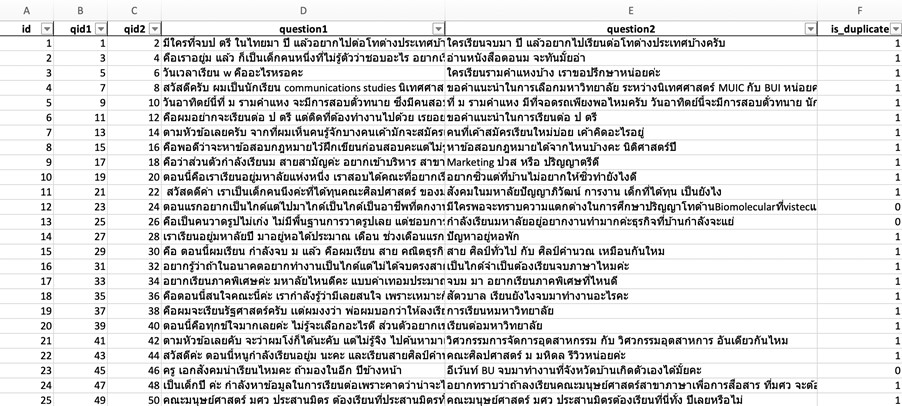
\includegraphics[width=14cm]{img/ch3/Example Data from Pantip.jpg}
	\caption{Example Data from Pantip}\label{fig:Example Data from Pantip}
\end{figure}

\begin{flushleft}
In our project, we try to do the NLP process in Thai language by tokenizing a chunk of Thai text into desirable units and building our dictionary to train data from Pantip.\\
Pre-processing data by trying to convert text it into lists of word indices or sequence. Then creating a function to remove specific characters and turn the word into embedding metric by word2vec a Thai vocabulary which is a dictionary that we build by ourselves and load by genism model where the keys are words (str) and values are the corresponding indices (a unique id as int).
\end{flushleft}

\begin{figure}[!h]
	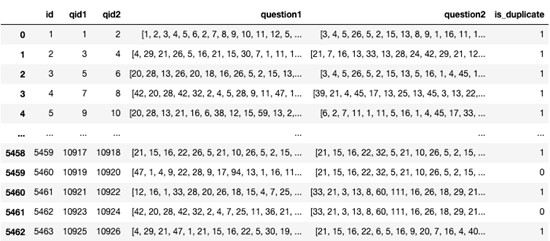
\includegraphics[width=14cm]{img/ch3/After preprocessing data by word2vec.jpg}
	\caption{After preprocessing data by word2vec}\label{fig:After preprocessing data by word2vec}
\end{figure}

\section{Design of key processing algorithms}
\begin{flushleft}
In the model prediction subsystem, we split our data into “left” and “right” inputs (one for each side of the MaLSTM) and Pad all the word number sequences with zeros. We also create a two thousand validation dataset to measure our model using the scikit learns train\_test\_split function. It can help to keeps the distribution of the label between the datasets by default.
\end{flushleft}

\pagebreak

\begin{figure}[!h]
	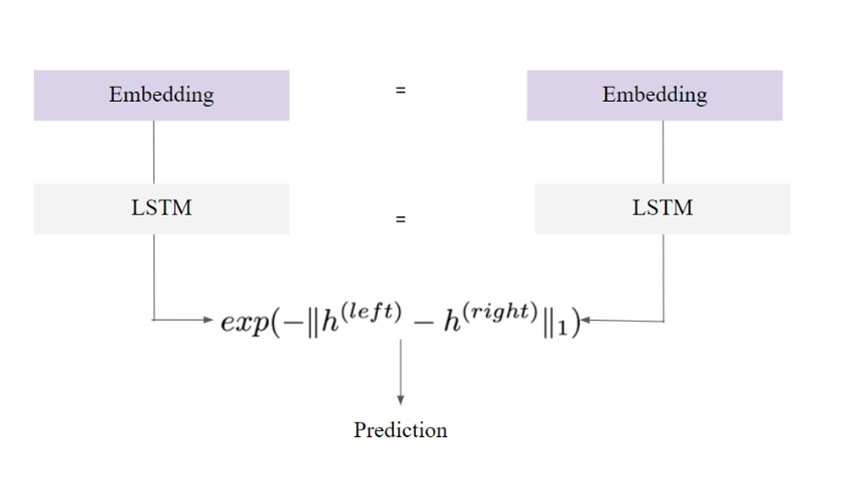
\includegraphics[width=14cm]{img/ch3/The architecture of Siamese neural network with MaLSTM for learning similarity.jpg}
	\caption{The architecture of Siamese neural network with MaLSTM for learning similarity}\label{fig:The architecture of Siamese neural network with MaLSTM for learning similarity}
\end{figure}

\begin{flushleft}
Two vectors hold the semantic meaning of each question and put them through the defined similarity function, since having an exponent of a negative the output. The prediction will return between 0 and 1. (1 refers to maximum similarity, and 0 refers to minimum similarity).\\
 Input to the network is zero-padded sequences of word indices. These inputs are vectors of fixed length, where the first zeros are being ignored, and the nonzero is indices that uniquely identify words. Those vectors are fed into the embedding layer. This layer looks up the corresponding embedding for each word and encapsulates all of them into a matrix. This matrix represents the given text as a series of embeddings.\\
Prepare from the pre-processing process, which are two embedded matrices representing a candidate of two related questions and create the helper function for the similarity estimate of the LSTMs outputs. Then feed them into the LSTM, and the final state of the LSTM for each question is a 50-dimensional vector then, train the model with 25 epochs and use batch sizes 64. We trained the model to capture the semantic meaning of the question, and the optimizer that we choose is the Adadelta optimizer and uses gradient clipping to avoid the exploding gradient problem.
\end{flushleft}

\begin{figure}[!h]
	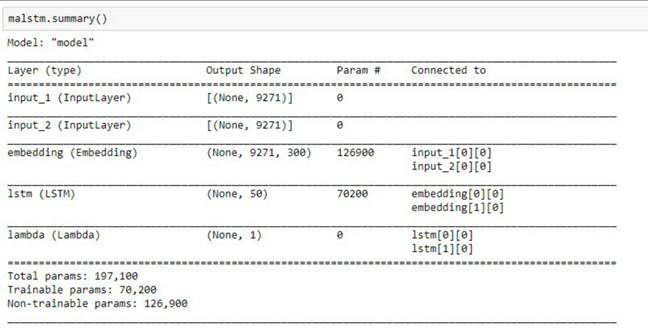
\includegraphics[width=14cm]{img/ch3/Model Summary.jpg}
	\caption{Model Summary}\label{fig:Model Summary}
\end{figure}

\pagebreak

\section{Evaluation plans}
\begin{itemize}
  \item Overall requirements
\begin{flushleft}
Our system can reply and answer the question from people who asked via Facebook Messenger automatically. In addition to satisfying score and comment from people who have used.
\end{flushleft}

  \item Knowledge Management
\begin{table}[h]
	\caption{Evaluation knowledge management table}
	\label{tab:Evaluation knowledge management table}
\begin{adjustbox}{width=\textwidth}
\begin{tabular}{|p{0.3\linewidth}|p{0.2\linewidth}|p{0.5\linewidth}|p{0.1\linewidth}|}
\hline
\rowcolor[HTML]{C9DAF8} 
Features                             & Role                    & Function                           & Status \\ \hline
                                     & Admin                   & Login                              &        \\ \cline{2-4} 
                                     & Admin                   & Logout                             &        \\ \cline{2-4} 
\multirow{-3}{*}{Account}            & Admin                   & Edit profile                       &        \\ \hline
                                     &                         & Create new category                &        \\ \cline{3-4} 
                                     &                         & Remove category                    &        \\ \cline{3-4} 
\multirow{-3}{*}{Manage category}    & \multirow{-3}{*}{Admin} & Update category                    &        \\ \hline
                                     &                         & Create new subcategory in category &        \\ \cline{3-4} 
                                     &                         & Remove subcategory                 &        \\ \cline{3-4} 
\multirow{-3}{*}{Manage subcategory} & \multirow{-3}{*}{Admin} & Update subcategory                 &        \\ \hline
                                     &                         & Create new FAQ                     &        \\ \cline{3-4} 
                                     &                         & Remove FAQ                         &        \\ \cline{3-4} 
\multirow{-3}{*}{Manage FAQ}         & \multirow{-3}{*}{Admin} & Update FAQ                         &        \\ \hline
                                     &                         & Create new user                    &        \\ \cline{3-4} 
                                     &                         & Remove user                        &        \\ \cline{3-4} 
\multirow{-3}{*}{Manage   user}      & \multirow{-3}{*}{Admin} & Update user                        &        \\ \hline
\end{tabular}
\end{adjustbox}
\end{table}


  \item Prediction Model
\begin{flushleft}
To evaluate prediction model base on different criteria for example accuracy and loss criteria, we plot training data vs validation data accuracy and loss and how the model can predict question.
\end{flushleft}
\end{itemize}

%%%%%%%%%%%%%%%%%%%%%%%%%%%%%%%%%%%%%%%%%%%%%%%%%%%%%%%%%%%%%%
%%%%%%%%%%%%%%%%%%%% Experiments %%%%%%%%%%%%%%%%%%%%%%%%%%%%%
%%%%%%%%%%%%%%%%%%%%%%%%%%%%%%%%%%%%%%%%%%%%%%%%%%%%%%%%%%%%%%%
\chapter{Implementation Results}
\section{Chatbot Subsystem Results}
Now our chatbot subsystem, we implemented in dialogflow which can classify greeting and understanding what is the questions. We also finished to implement SSL and DNS server on Cloudflare.

\begin{figure}[!h]\centering
\fbox{
\includegraphics[width=14cm]{./img/ch4/ch4_1.png}}
\caption{Classification greeting messages and questions}\label{fig:Classification greeting messages and questions}
\end{figure}
\begin{figure}[!h]\centering
\fbox{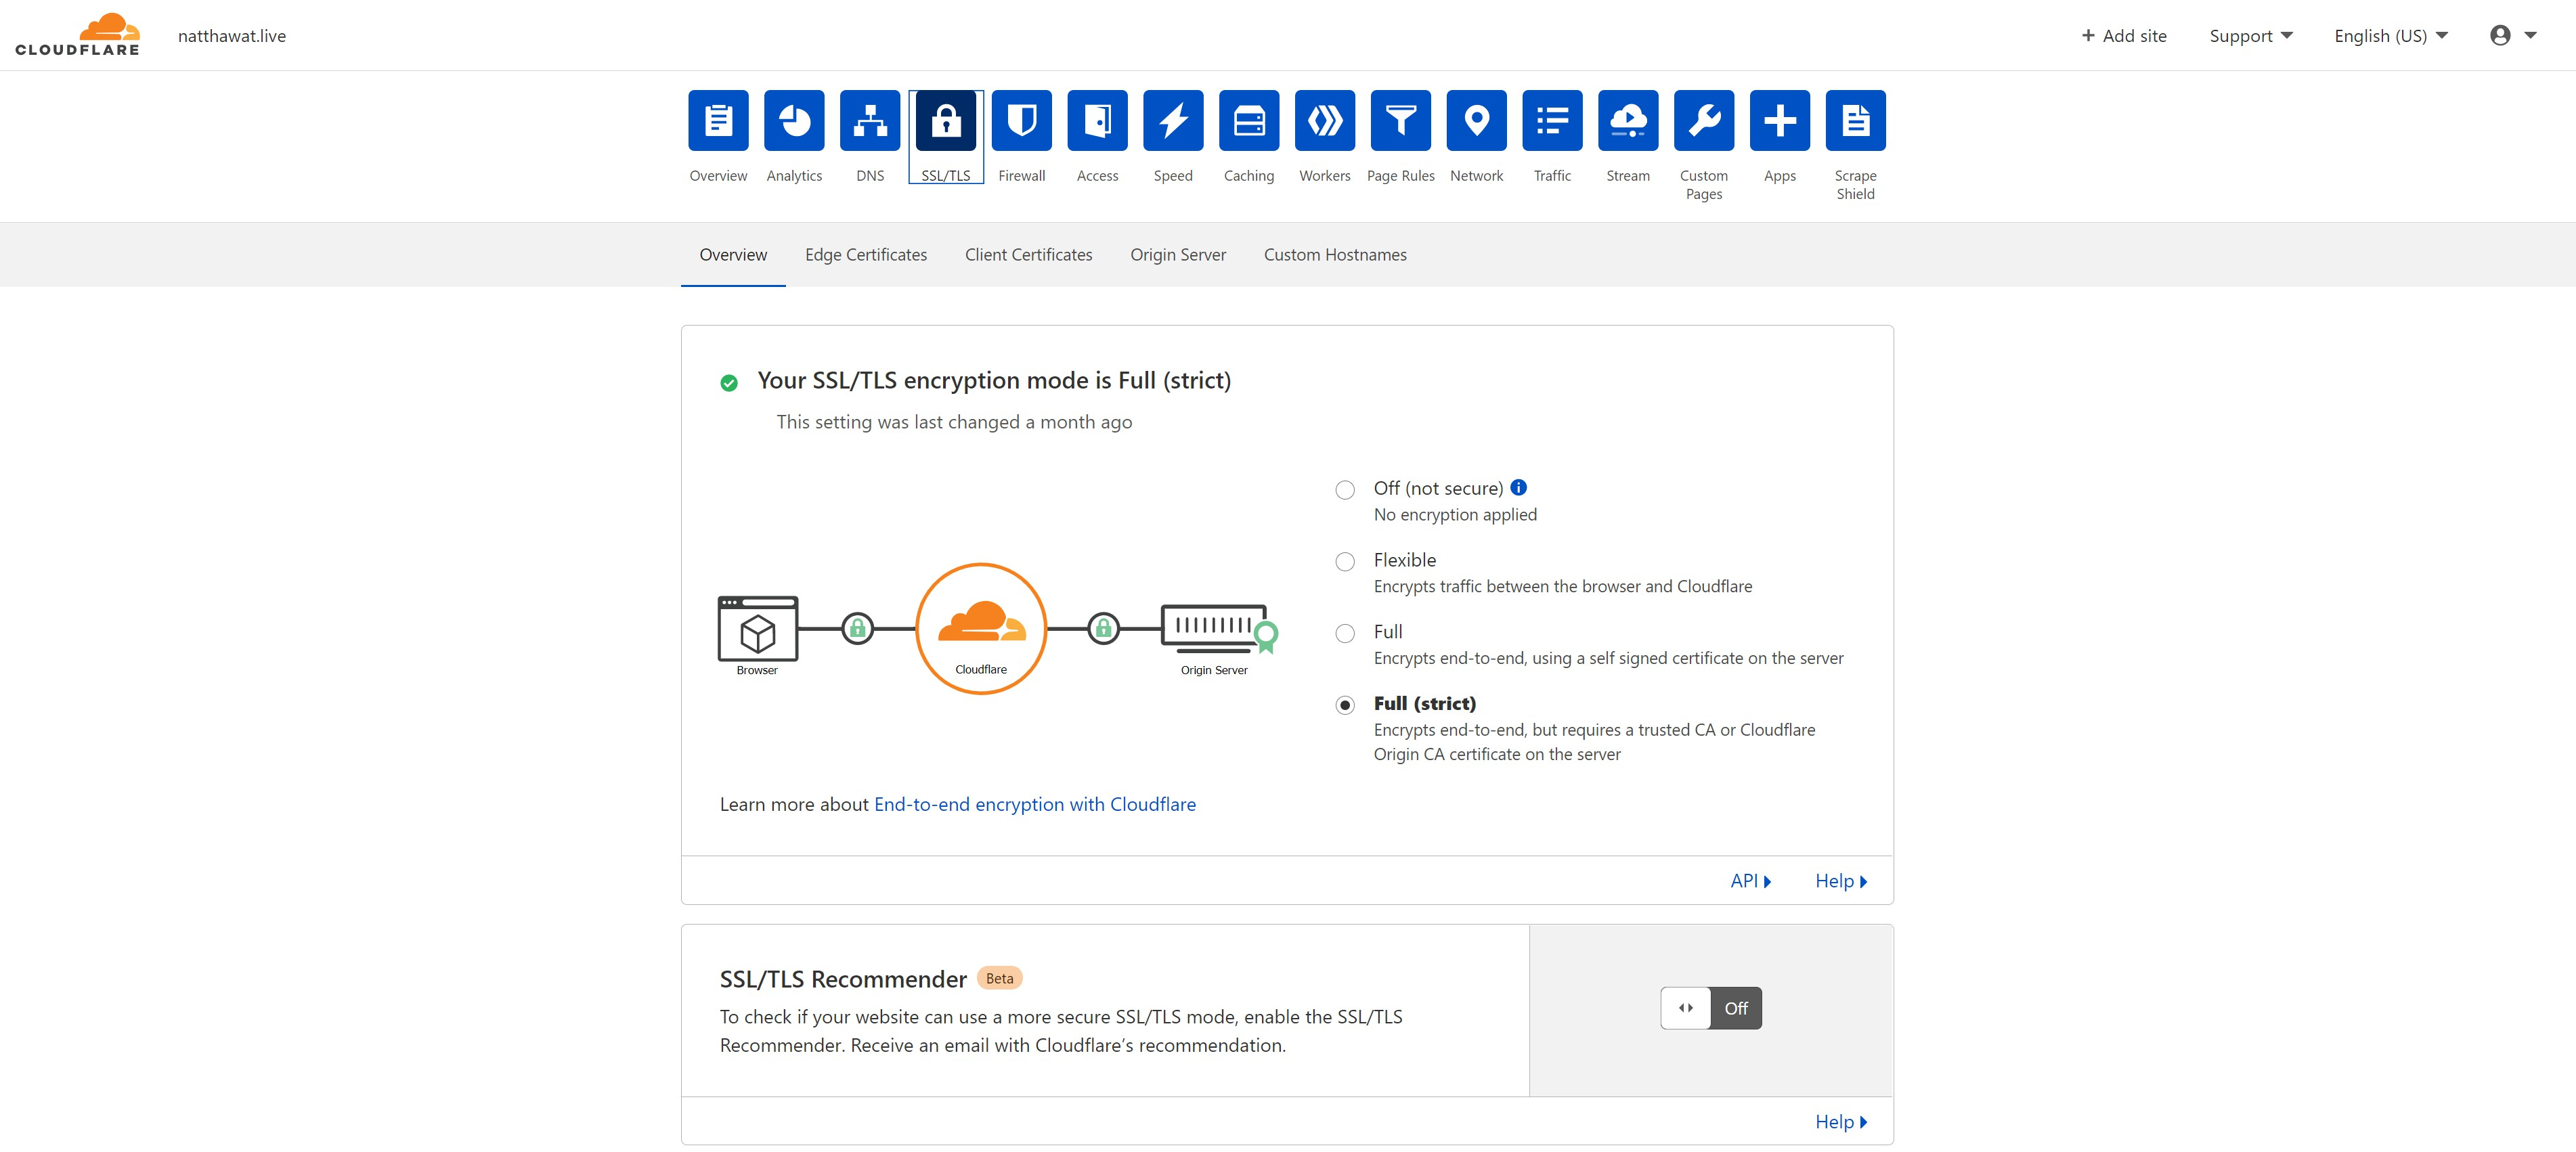
\includegraphics[width=14cm]{./img/ch4/ch4_Cloudflare.jpg}}
\caption{The SSL and DNS server of KMUTT CPE chatbot system on Cloudflare}\label{fig:The SSL and DNS server of KMOTT CPE chatbot system on Cloudflare}
\end{figure}


\section{Storage Subsystem Results}
For storage subsystem, we have already prepared the environment and dependency and implemented the restful API and graphQL for all subsystems. Now our system can create, update, delete, and query category, subcategory, users, and FAQs.
\begin{figure}[!h]\centering
\fbox{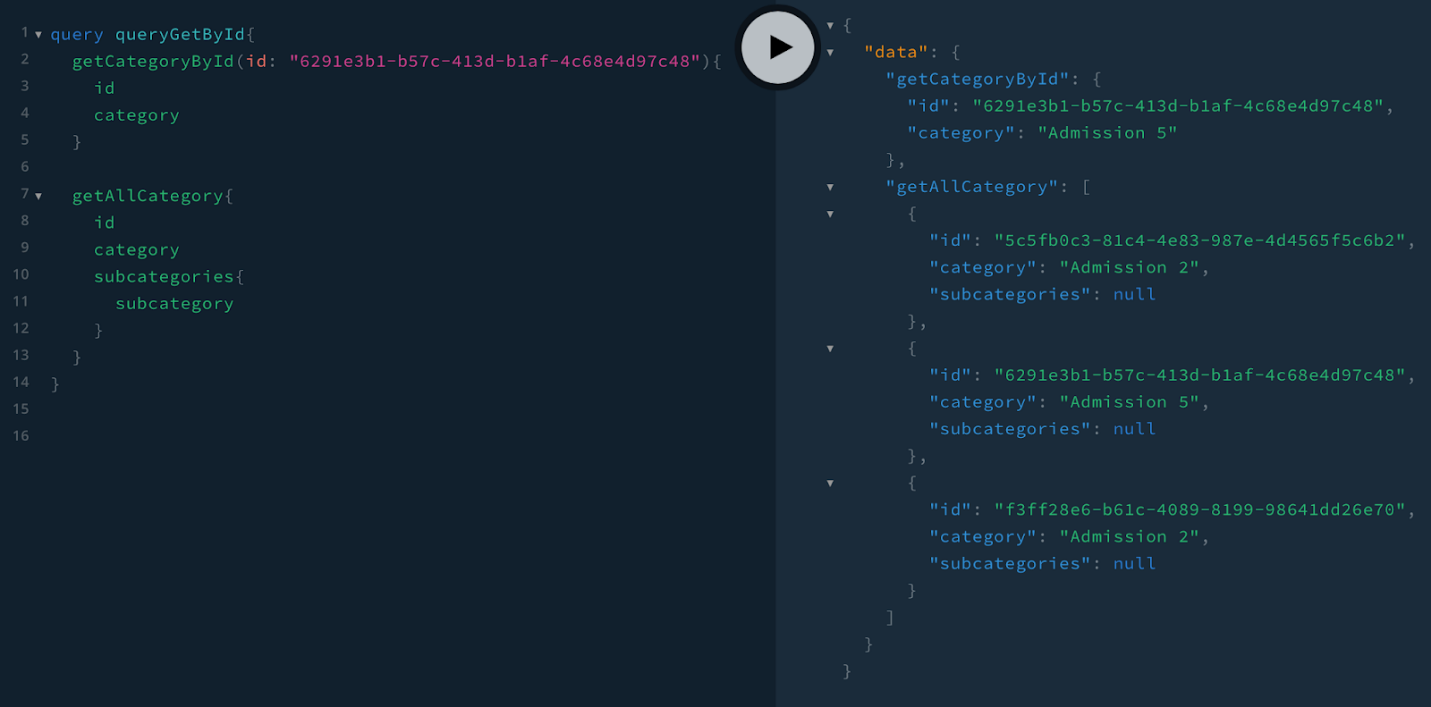
\includegraphics[width= 14cm]{./img/ch4/ch4_2.png}}
\caption{GraphQL query FAQs by ID category from backend API}\label{fig:GraphQL query FAQs category from backend API}
\end{figure}
\begin{figure}[!h]\centering
\fbox{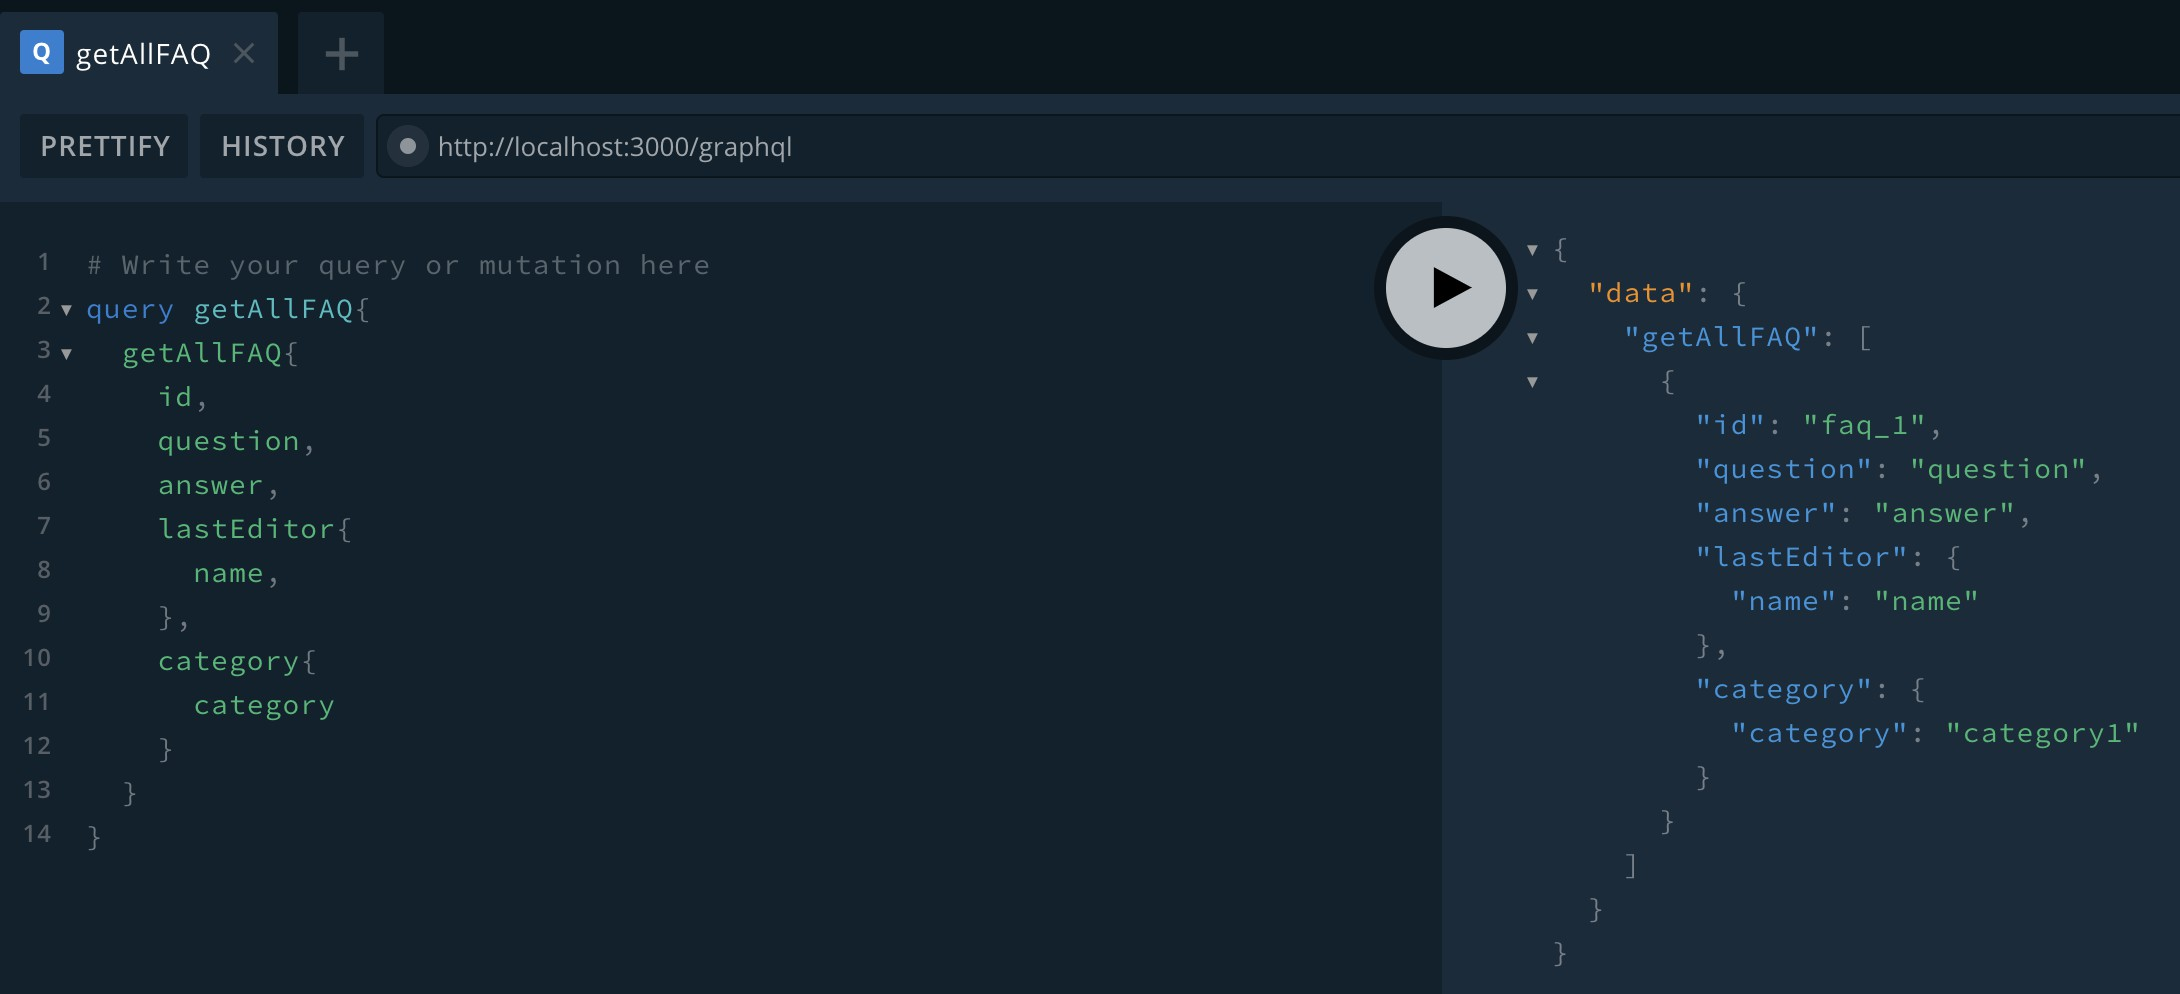
\includegraphics[width= 14cm]{./img/ch4/ch4_GetFAQ.jpg}}
\caption{GraphQL query FAQs from backend API}\label{fig:GraphQL query FAQs from backend API}
\end{figure}
\begin{figure}[!h]\centering
\fbox{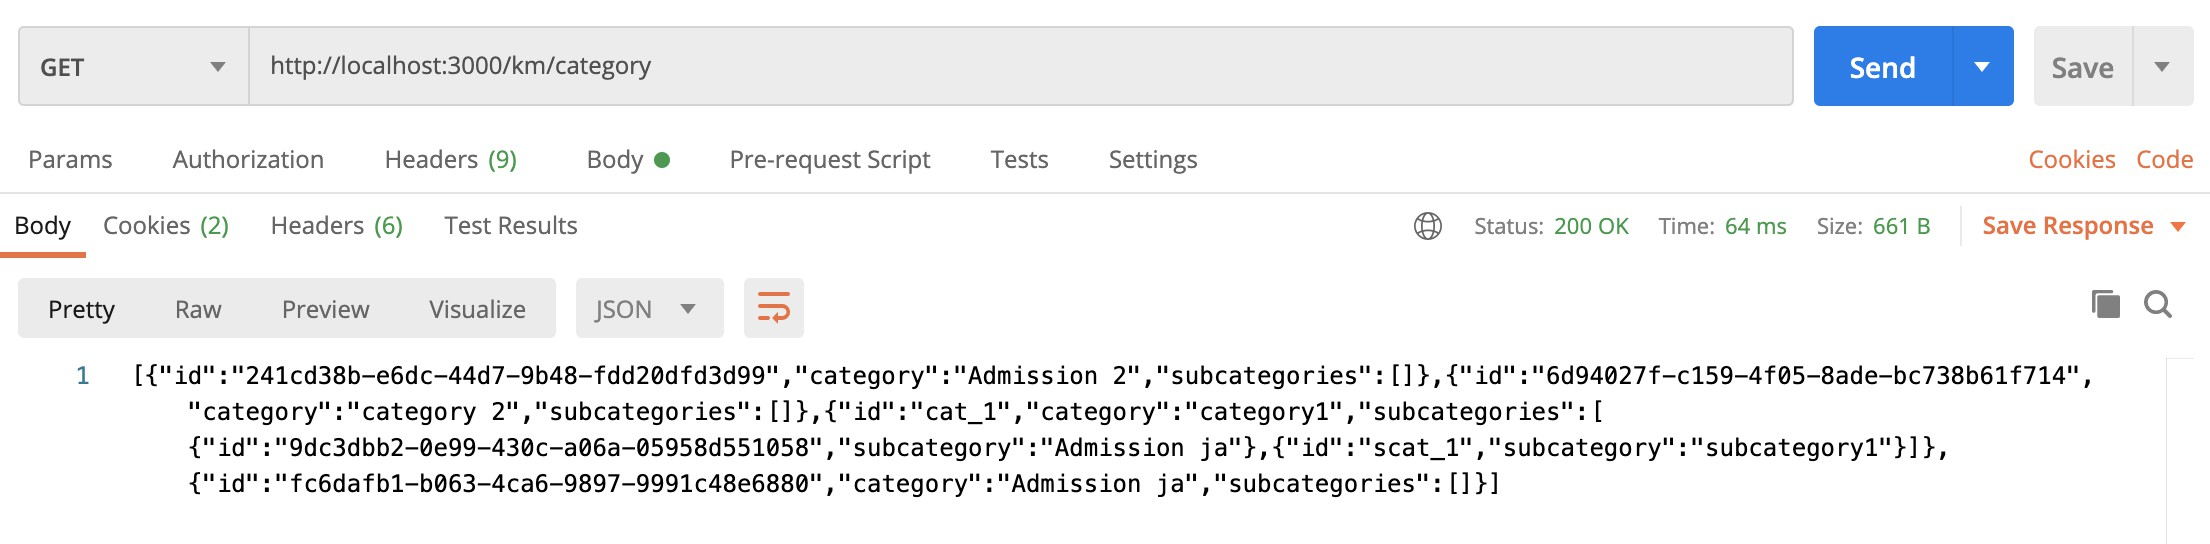
\includegraphics[width= 14cm]{./img/ch4/chap4_get.jpg}}
\caption{The result from Rest API by using GET Method to query category}\label{fig:The result from Rest API by using GET Method to query category}
\end{figure}

\section{Model Prediction Subsystem Results}
\subsection{Training Siamese Neural Network with MaLSTM Result}
After preprocessing the data, we split the data into train, validate, and test data. Then separate the data into left inputs and right inputs, one for each side of MaLSTM. Then train the model with 100 epochs and use batch sizes 128. In addition to using early stops to prevent the model too overfitting and model checkpoint to save the model. Even our group set 100 epochs, but the model was trained only 17 epochs before stopping from early stop. Loss of training data is 0.4116 and loss of validation data is 0.4358. Also, accuracy of training data is 0.5487 and accuracy of validation data is 0.4358. Graphs below are the result from training.

\begin{figure}[!h]\centering
\fbox{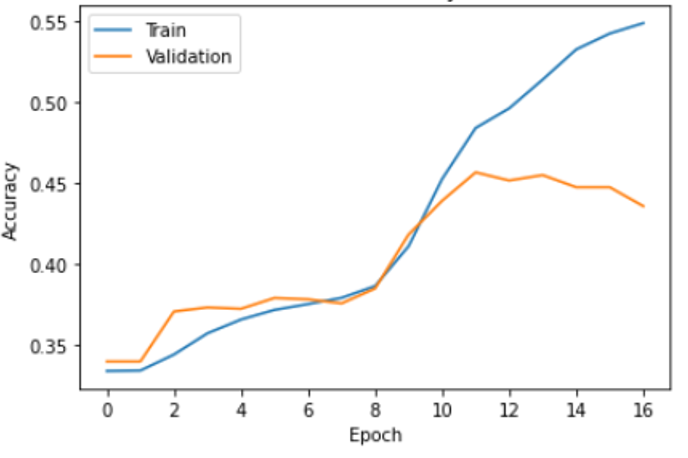
\includegraphics[width= 14cm]{./img/ch4/ch4_3.png}}
\caption{Model accuracy}\label{fig:Model accuracy}
\end{figure}
\begin{figure}[!h]\centering
\fbox{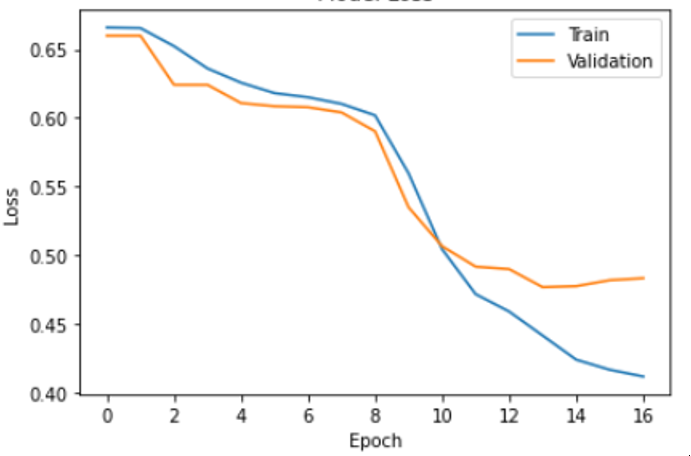
\includegraphics[width= 14cm]{./img/ch4/ch4_4.png}}
\caption{Model loss}\label{fig:Model loss}
\end{figure}

\subsection{Evaluation Model Result}
The result from the model is the real number from 0 to 1. We interpret both questions are similar (result = 1) if the model predicted score is more than 0.3. If the model predicted score is less than 0.3, both questions are not similar (result = 0). We pick 0.3 to be a criterion for similar or not similar because we have picked 0.6 and 0.5 already but accuracy is very low. After the model predicts the test data, we convert from a similar score (0 to 1)  to binary (0 or 1) instead before evaluating. As you can see in the training topic, we use accuracy and loss to be the main criteria to evaluate the model while training. But in this process we will also use accuracy, precision, and F1-score to evaluate the model. The picture below is the result after evaluating the model with test data.

\begin{figure}[!h]\centering
\fbox{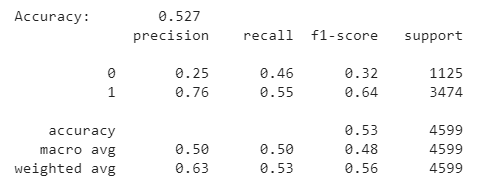
\includegraphics[width= 14cm]{./img/ch4/ch4_5.png}}
\caption{Classification report}\label{fig:Classification report}
\end{figure}
\begin{figure}[!h]\centering
\fbox{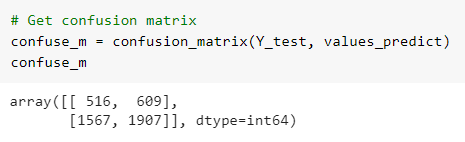
\includegraphics[width= 14cm]{./img/ch4/ch4_6.png}}
\caption{Confusion matrix}\label{fig:Confusion matrix}
\end{figure}

The accuracy after evaluating with test data is 0.527. From the confusion matrix and classification report, the overall model performs accuracy with 52.7\%. There are two classes and we got class o with less precision around 25\%. but we have got class 1 with high precision with 76\%.
\subsection{Siamese Neural Network with MaLSTM Model Result}

The picture below shows an example result from playing with the model. The Input questions are
{
\XeTeXlinebreaklocale "th_TH"	
\thaifont 
'วิศวะคอมเรียนหลักสูตรอะไรบ้างคะ' }
and
{
\XeTeXlinebreaklocale "th_TH"	
\thaifont 
 ' วิศวะคอมมีหลักสูตรอะไรบ้าง'. 
}Both questions are similar and our model can predict both questions are similar for 83.33\%.

\begin{figure}[!h]\centering
\fbox{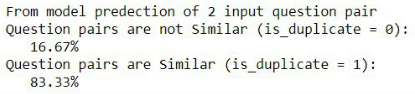
\includegraphics[width= 14cm]{./img/ch4/ch4_7.png}}
\caption{Model result by compare questions which similar}\label{fig:Model result by compare questions which similar}
\end{figure}

From others example from playing with model.The Input questions are
{
\XeTeXlinebreaklocale "th_TH"	
\thaifont 
 ‘ วิศวะคอมเรียนเกี่ยวกับอะไรบ้าง’ }and 
{
\XeTeXlinebreaklocale "th_TH"	
\thaifont ‘ วิศวะคอมมีเรียนหลักสูตรอะไรบ้าง’.}
 Both questions are not similar and our model can predict both questions are not similar for 57.14\%

\begin{figure}[!h]\centering
\fbox{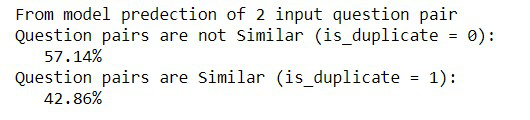
\includegraphics[width= 14cm]{./img/ch4/ch4_8.png}}
\caption{Model result by compare questions which not similar}\label{fig:Model result by compare questions which not similar}
\end{figure}

Even the model can predict, but the overall performance of the model is quite not good. Because we think the model should return similar questions from MaLSTM more than 0.5 scores not 0.3 scores. We think that the problem comes from not enough data. If we can gather more dataset and have more cases about question pairs that are similar or not similar, especially not similar that we got less precision, we can increase our model's performance. Also we have to integrate all subsystem to be one system in the production environment.

%%%%%%%%%%%%%%%%%%%%%%%%%%%%%%%%%%%%%%%%%%%%%%%%%%%%%%%%%%%%%%%
%%%%%%%%%%%%%%%%%%%% Conclusions %%%%%%%%%%%%%%%%%%%%%%%%%%%%%
%%%%%%%%%%%%%%%%%%%%%%%%%%%%%%%%%%%%%%%%%%%%%%%%%%%%%%%%%%%%%%%
% \chapter{Conclusions}

% This chapter is optional for proposal and progress reports but 
% is required for the final report.

% \section{Problems and Solutions}
% State your problems and how you fixed them.

% \section{Future Works}
% What could be done in the future to make your projects better.

%%%%%%%%%%%%%%%%%%%%%%%%%%%%%%%%%%%%%%%%%%%%%%%%%%%%%%%%%%%%%%%
%%%%%%%%%%%%%%%%%%%% Bibliography %%%%%%%%%%%%%%%%%%%%%%%%%%%%%
%%%%%%%%%%%%%%%%%%%%%%%%%%%%%%%%%%%%%%%%%%%%%%%%%%%%%%%%%%%%%%%

%%%% Comment this in your report to show only references you have
%%%% cited. Otherwise, all the references below will be shown.
\nocite{*}
%% Use the kmutt.bst for bibtex bibliography style 
%% You must have cpe.bib and string.bib in your current directory.
%% You may go to file .bbl to manually edit the bib items.
\bibliographystyle{kmutt}
\bibliography{string,cpe}

%%%%%%%%%%%%%%%%%%%%%%%%%%%%%%%%%%%%%%%%%%%%%%%%%%%%%%%%%%%%%%%
%%%%%%%%%%%%%%%%%%%%%%%% Appendix %%%%%%%%%%%%%%%%%%%%%%%%%%%%%
%%%%%%%%%%%%%%%%%%%%%%%%%%%%%%%%%%%%%%%%%%%%%%%%%%%%%%%%%%%%%%%
% \appendix{First appendix title}
% \noindent{\large\bf Put appropriate topic here} \\

% This is where you put hardware circuit diagrams, detailed experimental data in tables or source codes, etc.. \\ \bigskip



% This appendix describes two static allocation methods for fGn (or fBm)
% traffic. Here, $\lambda$ and $C$ are respectively the traffic arrival
% rate and the service rate per dimensionless time step. Their unit are
% converted to a physical time unit by multiplying the step size
% $\Delta$. For a fBm self-similar traffic source,
% Norros~\cite{norros95} provides its EB as
% \begin{equation}\label{eq:norros}
%   C = \lambda + (\kappa(H)\sqrt{-2\ln\epsilon})^{1/H}a^{1/(2H)}x^{-(1-H)/H}\lambda^{1/(2H)}
% \end{equation}
% where $\kappa(H) = H^H(1-H)^{(1-H)}$. Simplicity in the calculation is
% the attractive feature of (\ref*{eq:norros}).

% The MVA technique developed in~\cite{kim01} so far provides the most
% accurate estimation of the loss probability compared to previous
% bandwidth allocation techniques according to simulation results.
% Consider a discrete-time queueing system with constant service rate
% $C$ and input process $\lambda_n$ with $\mathbb{E}\{\lambda_n\} =
% \lambda$ and $\mathrm{Var}\{\lambda_n\} = \sigma^2$.  Define $X_n \equiv
% \sum_{k=1}^n \lambda_k - Cn$.  The loss probability due to the MVA
% approach is given by
% \begin{equation}\label{eq:loss_mva}
%   \varepsilon \approx \alpha e^{-m_x/2}
% \end{equation}
% where
% \begin{equation}\label{eq:mx}
% m_x = \min_{n \geq 0} \frac{((C-\lambda)n + B)^2}{\mathrm{Var}\{X_n\}} =
% \frac{((C-\lambda)n^\ast + B)^2}{\mathrm{Var}\{X_{n^{\ast}}\}}
% \end{equation} 
% and 
% \begin{equation}\label{eq:alpha}
%   \alpha =
%   \frac{1}{\lambda\sqrt{2\pi\sigma^2}}\exp\left(\frac{(C-\lambda)^2}{2\sigma^2}\right)
%   \int_C^\infty (r-C)\exp\left(\frac{(r-\lambda)^2}{2\sigma^2}\right)\, dr
% \end{equation}
% For a given $\varepsilon$, we numerically solve for $C$ that satisfies
% (\ref*{eq:loss_mva}). Any search algorithm can be used to do the task.
% Here, the bisection method is used.  

% Next, we show how $\mathrm{Var}\{X_n\}$ can be determined.  Let
% $C_{\lambda}(l)$ be the autocovariance function of $\lambda_n$.  The
% MVA technique basically approximates the input process $\lambda_n$
% with a Gaussian process, which allows $\mathrm{Var}\{X_n\}$ to be
% represented by the autocovariance function.  In particular, the
% variance of $X_n$ can be expressed in terms of $C_{\lambda}(l)$ as
% \begin{equation}
%   \mathrm{Var}\{X_n\} = nC_{\lambda}(0) + 2\sum_{l=1}^{n-1} (n-l)C_{\lambda}(l)
% \end{equation} 
% Therefore, $C_{\lambda}(l)$ must be known in the MVA technique, either
% by assuming specific traffic models or by off-line analysis in case of
% traces.  In most practical situations, $C_{\lambda}(l)$ will not be
% known in advance, and an on-line measurement algorithm developed
% in~\cite{eun01} is required to jointly determine both $n^\ast$ and
% $m_x$. For fGn traffic, $\mathrm{Var}\{X_n\}$ is equal to $\sigma^2
% n^{2H}$, where $\sigma^2 = \mathrm{Var}\{\lambda_n\}$, and we can find
% the $n^\ast$ that minimizes (\ref*{eq:mx}) directly. Although $\lambda$
% can be easily measured, it is not the case for $\sigma^2$ and $H$.
% Consequently, the MVA technique suffers from the need of prior
% knowledge traffic parameters.


%%%%%%%%%%%%%%%%%%%%%%%%%%%%%%%%%%%%%%%%%%%%%%%%%%%%%%%%%%
%%%%%%%%%%%%%%% The 2nd appendix %%%%%%%%%%%%%%%%%%%%%%%%%%
%%%%%%%%%%%%%%%%%%%%%%%%%%%%%%%%%%%%%%%%%%%%%%%%%%%%%%%%%%
% \appendix{Second appendix title}
% \noindent{\large\bf Put appropriate topic here} \\

% Next, we show how $\mathrm{Var}\{X_n\}$ can be determined.  Let
% $C_{\lambda}(l)$ be the autocovariance function of $\lambda_n$.  The
% MVA technique basically approximates the input process $\lambda_n$
% with a Gaussian process, which allows $\mathrm{Var}\{X_n\}$ to be
% represented by the autocovariance function.  In particular, the
% variance of $X_n$ can be expressed in terms of $C_{\lambda}(l)$ as
% \begin{equation}
%   \mathrm{Var}\{X_n\} = nC_{\lambda}(0) + 2\sum_{l=1}^{n-1} (n-l)C_{\lambda}(l)
% \end{equation} 

% \noindent{\large\bf Add more topic as you need} \\

% Therefore, $C_{\lambda}(l)$ must be known in the MVA technique, either
% by assuming specific traffic models or by off-line analysis in case of
% traces.  In most practical situations, $C_{\lambda}(l)$ will not be
% known in advance, and an on-line measurement algorithm developed
% in~\cite{eun01} is required to jointly determine both $n^\ast$ and
% $m_x$. For fGn traffic, $\mathrm{Var}\{X_n\}$ is equal to $\sigma^2
% n^{2H}$, where $\sigma^2 = \mathrm{Var}\{\lambda_n\}$, and we can find
% the $n^\ast$ that minimizes (\ref*{eq:mx}) directly. Although $\lambda$
% can be easily measured, it is not the case for $\sigma^2$ and $H$.
% Consequently, the MVA technique suffers from the need of prior
% knowledge traffic parameters.





\end{document}
